\documentclass[11pt,a4paper]{article}
\usepackage[margin=20mm]{geometry}
\usepackage[T1]{fontenc}
\usepackage{lmodern,amsmath,amssymb,booktabs,graphicx,float,microtype}
\usepackage[hidelinks]{hyperref}
\usepackage[font=small,skip=5pt]{caption}
\hypersetup{pdftitle={DSA5208 Project 3: Parallel Urban Pollutant Transport},pdfauthor={Navneet Melarkode and Tridiv Swain}}
\setlength{\intextsep}{6pt}
\setlength{\textfloatsep}{8pt}
\setlength{\parskip}{3pt}\setlength{\parindent}{0pt}
\graphicspath{{figures/}}
\title{DSA5208 Project 3\\Parallel Urban Pollutant Transport\\\large Finite-volume and Lagrangian methods with MPI and Kokkos}
\author{Navneet Melarkode (A0326423L)\\Tridiv Swain (A0328390B)}
\date{}
\begin{document}
\maketitle
\vspace{-7mm}
\begin{abstract}
We built serial and MPI--Kokkos OpenMP solvers for pollutant dispersion using a grid and particles. The main challenges were boundary exchange, particle migration and load balance. The grid solver achieved $4.95\times$ speedup over serial on 12 Atlas cores and $2.40\times$ over a one-node MPI run on four Vanda nodes. Atlas multi-node timings varied more. Particles reached $13.1\times$ speedup (82\%) over the one-rank/one-thread parallel baseline on 16 Vanda cores; a compact plume produced a $13.2\times$ maximum-to-mean load ratio. In a 600 s urban experiment, the grid retained 1.395\% of the release and the three-seed particle mean retained 1.554\%. Grouping output into roughly 19 m columns revealed similar broad plume patterns. We discuss the numerical checks, performance and limits of the urban model.
\end{abstract}

\section{Transport model and numerical methods}
We prescribe a stationary wind $\mathbf u$ and constant diffusivity $K$, represent buildings as solid cells, and release a Gaussian pollutant cloud once. There are no reactions, deposition or later sources:
\begin{equation}
\partial_t c+\nabla\!\cdot(\mathbf u c)=K\nabla^2c,
\qquad M(t)+M_{\rm escaped}(t)=M_0=1.
\end{equation}
We normalize the released mass to one. Each grid update needs neighbouring concentrations, while particles cross rank boundaries and can cluster on a few ranks. These dependencies make parallel communication and load balance central to the project.

\textbf{Finite volume.} For adjacent air cells $i,j$, outward normal velocity $u_f$ and spacing $h_f$, we use upwind advection, centered diffusion and forward Euler:
\begin{equation}
F_{ij}=\max(u_f,0)c_i+\min(u_f,0)c_j-K\frac{c_j-c_i}{h_f},\qquad
c_i^{n+1}=c_i^n-\frac{\Delta t}{V_i}\sum_f A_fF_{if}^n.
\end{equation}
Shared face fluxes cancel in the total mass sum. We average cell velocities at faces and set flux to zero at solids and closed boundaries. Open boundaries admit clean air, track advective escape and have zero diffusive flux. We integrate the initial Gaussian over cells and normalize it over air. The timestep satisfies $\Delta t\leq\mathrm{CFL}/\max_i\lambda_i$, where $\lambda_i$ includes outgoing advection and diffusion; urban CFL is 0.8. The solver rejects unsafe timesteps and updates concentrations without clipping. Prescribed wind still requires this stability check.

\textbf{Particles.} Each particle carries mass $1/N$. In uniform unbounded flow,
\begin{equation}
\mathbf X^{n+1}=\mathbf X^n+\mathbf u\Delta t+\sqrt{2K\Delta t}\,\boldsymbol\xi^n,
\qquad \boldsymbol\xi^n\sim\mathcal N(\mathbf0,I).
\end{equation}
Philox uses the seed, global particle ID, timestep and stream index to generate random increments \cite{random123}. Each particle keeps its stream when it moves between MPI ranks. We assign particle mass to the cell containing it and sample initial urban positions from the Gaussian over available air.

\textbf{Shared urban physics.} We reconstruct particle velocity linearly from the same normal face velocities used by the grid. Drift is followed by diffusion: drift may leave open boundaries, while diffusion reflects there to match zero diffusive flux. Both reflect at solids and closed boundaries. A cell-by-cell segment walk detects wall crossings. Particles wrap at periodic boundaries and change owner at MPI boundaries. Splitting, reflection and velocity reconstruction introduce differences between the two methods. Both use the prescribed wind without a divergence-free projection.
\clearpage

\section{Parallel design}
\textbf{Grid decomposition.} We split the horizontal plane into slabs or blocks using MPI (Figure~\ref{fig:grid_partition}). Each rank keeps all vertical layers and exchanges one layer of cells with its face neighbours. This also works for uneven partitions and partitions only one cell wide. Kokkos handles updates and reductions within each rank. We compare two communication approaches. The blocking version finishes communication before updating cells. The overlap version starts communication, updates the interior, waits for the messages and then updates boundary cells. Blocks can reduce boundary area while increasing the number of neighbours. Thin partitions leave less interior work to overlap, and the benefit also depends on MPI communication progress.

\begin{figure}[H]\centering
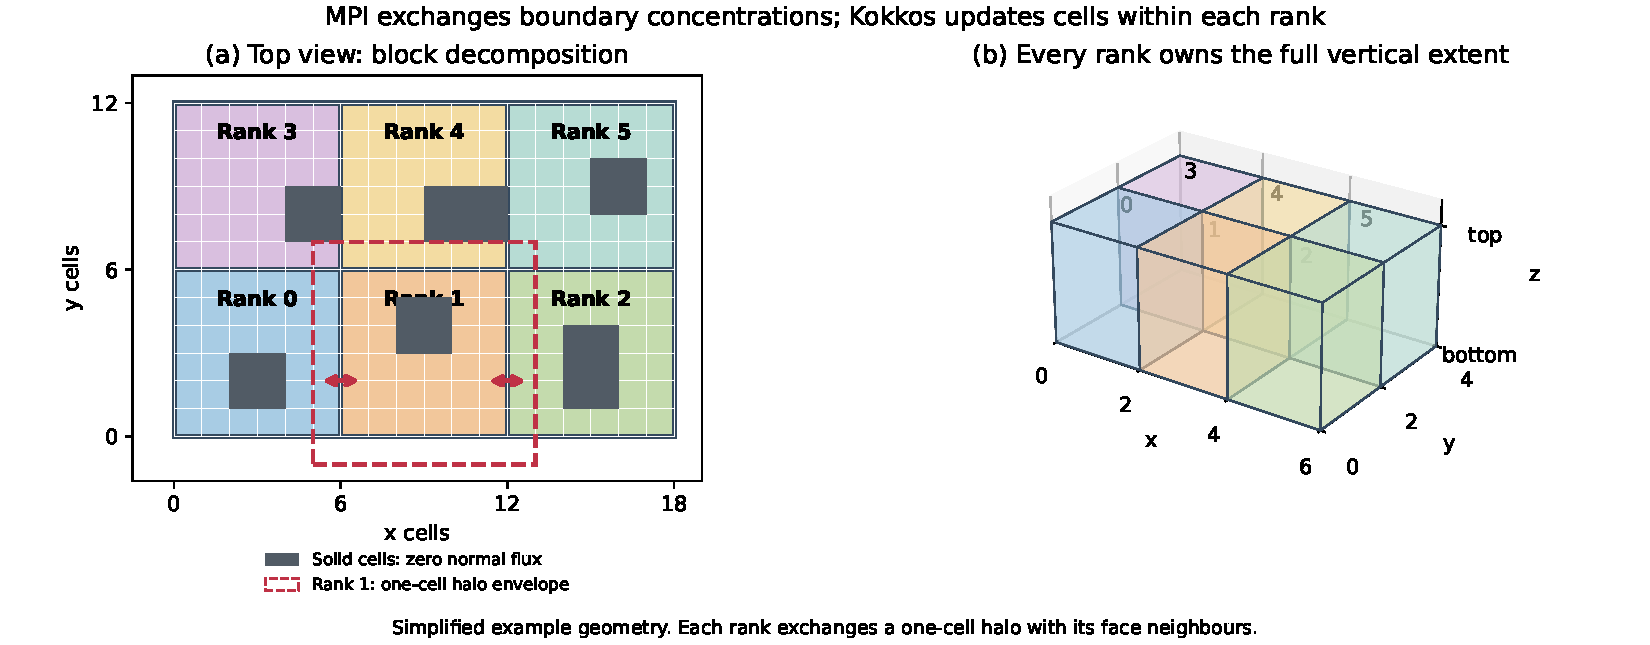
\includegraphics[width=\linewidth]{grid_partition.pdf}
\caption{A small example of grid ownership. Colours show MPI ranks and grey cells show solids. The red outlines mark rank 1's neighbouring face halos. The bottom lies on a physical domain boundary and uses its boundary condition. Each rank owns the full vertical column. We use this simplified geometry to explain the decomposition.}
\label{fig:grid_partition}
\end{figure}

\textbf{Particle decomposition.} We assign particles to ranks using a Cartesian decomposition and store their properties in separate arrays for Kokkos updates. After each complete physical step, \texttt{MPI\_Alltoallv} transfers particles directly to their final owner, including multi-subdomain jumps. IDs, positions, image counters, masses and active flags migrate together. We reduce local quantities across MPI ranks for diagnostics. Particle counts and an ID fingerprint provide checks during execution; validation dumps check that every ID appears exactly once.

The serial and parallel particle solvers share the same release and stepping routines. The grid solvers use separate steppers with shared coefficients and I/O. This makes comparison easier, although an error in shared code can affect both versions. Every particle rank loads the full wind and mask, and rank zero gathers concentration output. These choices simplify the implementation but limit scalability. A localized plume can also leave most ranks with little work.

\textbf{Design lesson.} We found that the best layout depends on where the work is. A broad particle cloud spreads work across ranks; a compact urban release can concentrate it on just a few. We therefore tested communication and thread choices for both situations.
\clearpage

\section{Correctness and single-node grid performance}
For the analytical Gaussian, $\boldsymbol\mu(t)=\mathbf x_0+\mathbf ut$ and $\sigma_d^2(t)=\sigma_0^2+2Kt$. Tests avoid unintended boundary interaction; Figure~\ref{fig:convergence} shows the measured convergence.
\begin{table}[H]\centering\small
\begin{tabular}{p{.25\linewidth}p{.68\linewidth}}\toprule
Evidence & Result \\\midrule
Grid, Atlas & 59 runs: analytical convergence, mass/positivity, stationary state, open budgets, walls, uneven partitions and serial/MPI equivalence passed. \\
Particles & 94 original unit checks; analytical moment checks over ten seeds; 72 MPI runs (6 cases $\times$ 12 layouts), 624 checks, passed in supplied Vanda evidence and an independent local rerun. Tested per-ID states matched serial exactly. \\
Urban integration & Ten refactor cases were byte-identical. Wall traversal, randomized reflections, I/O equivalence and sanitizer checks passed locally. \\
Full urban MPI replay & All 21 saved fields matched serial exactly for one 100,000-particle seed; diagnostics passed tolerances. \\
New multi-node runs & On each cluster, 18 saved-field comparisons and 18 measured runs passed, with checked placement, bindings, mass budgets and positivity. \\\bottomrule
\end{tabular}
\caption{These tests check the implementation and numerical behaviour. The wind and geometry require their own validation. Exact serial/MPI matches were observed for the builds and cases tested here.}
\end{table}
\begin{figure}[H]\centering
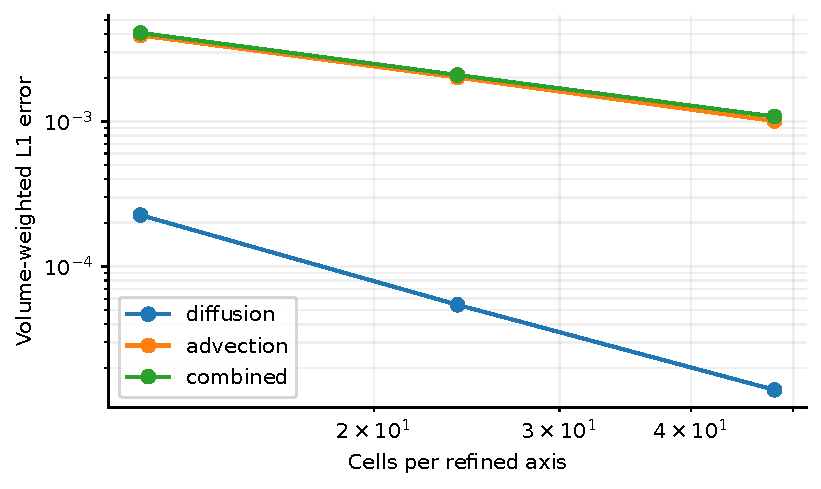
\includegraphics[width=.40\linewidth]{convergence.pdf}
\caption{Atlas refinement: approximately second-order diffusion and first-order advection; combined error is advection-dominated.}
\label{fig:convergence}
\end{figure}

Figure~\ref{fig:grid_scaling} compares the Atlas layouts. The benchmark uses $256\times256\times32$ cells, 100 steps of $\Delta t=0.5$ s, no concentration snapshots and three repeats. Serial median time is 1.36578 s. The best layout, 6 ranks $\times$ 2 threads with slab/blocking, takes 0.27569 s: $4.954\times$ speedup and 41.3\% efficiency. Its three repeats span 0.25384--0.30985 s. One-rank/one-thread slab/blocking takes 2.02142 s ($0.676\times$ serial speed), showing one-core parallel overhead. For the same 6-rank $\times$ 2-thread slab/blocking layout, the halo median is 0.09255 s. Memory bandwidth is another possible limit, but was not measured; the allocation's CPU model was not recorded.
\begin{figure}[H]\centering
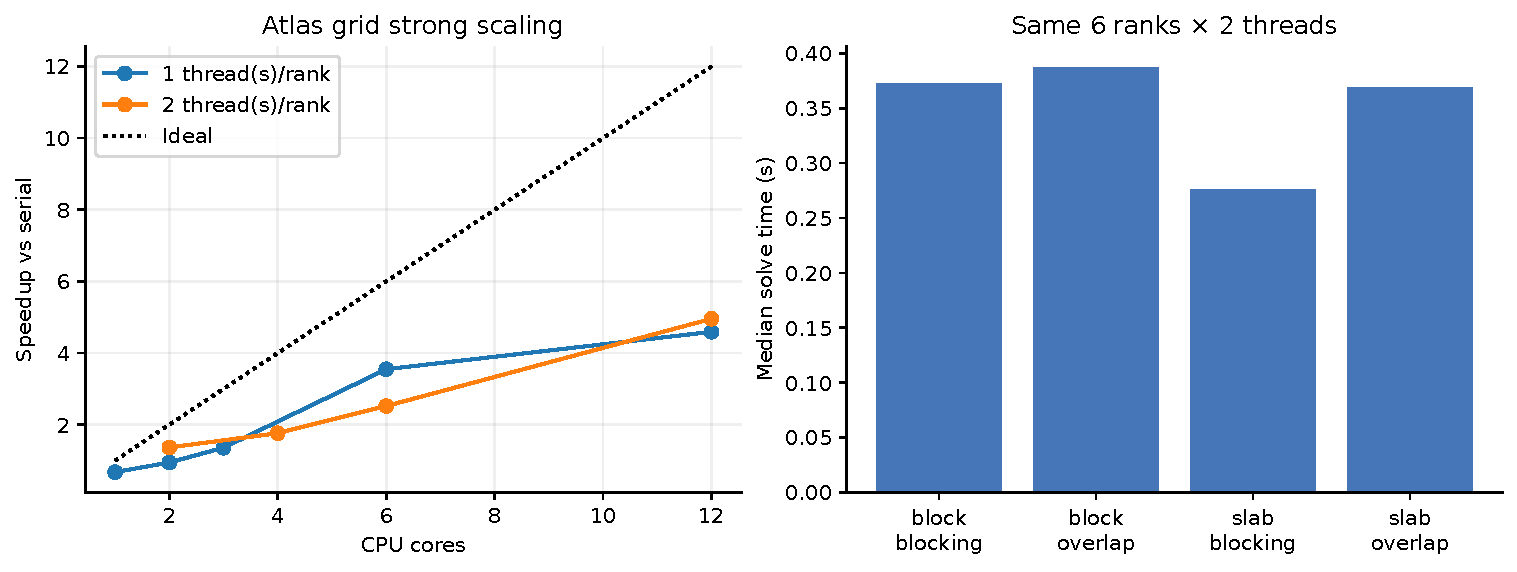
\includegraphics[width=.88\linewidth]{grid_scaling.pdf}
\caption{Single-node Atlas grid scaling and fixed-core layout choices. Here $S=T_{\rm serial}/T_p$ and $E=S/p$, with $p$ allocated cores. This baseline differs from the node-relative study below.}
\label{fig:grid_scaling}
\end{figure}
\clearpage

\section{Particle scaling and load imbalance}
Figure~\ref{fig:particle_scaling} shows the particle scaling results. These Vanda measurements used one dual Xeon Gold 6438N node (64 physical cores, at most 16 allocated), GCC 13.3, Open MPI 5.0.3 and Kokkos 4.7.04/OpenMP. A broad periodic cloud gives approximately balanced ownership. Strong scaling uses 10 million particles and 100 steps; weak scaling uses one million particles per core in the same physical domain.

For timing, we add stepping, waiting and migration on each rank, then take the largest total. Setup and output are excluded. The baseline is the one-rank/one-thread \emph{parallel} executable: 91.5187 s. At $4\times4$, the loop takes 6.98356 s: $13.1049\times$ speedup and 81.9\% efficiency. At 16 cores, hybrid weak efficiency is 82.2\%, versus 74.8\% for pure MPI. Each configuration has only one observation. A matching serial timing for this 10-million-particle workload was not recorded, so these speedups describe scaling within the parallel executable.
\begin{figure}[H]\centering
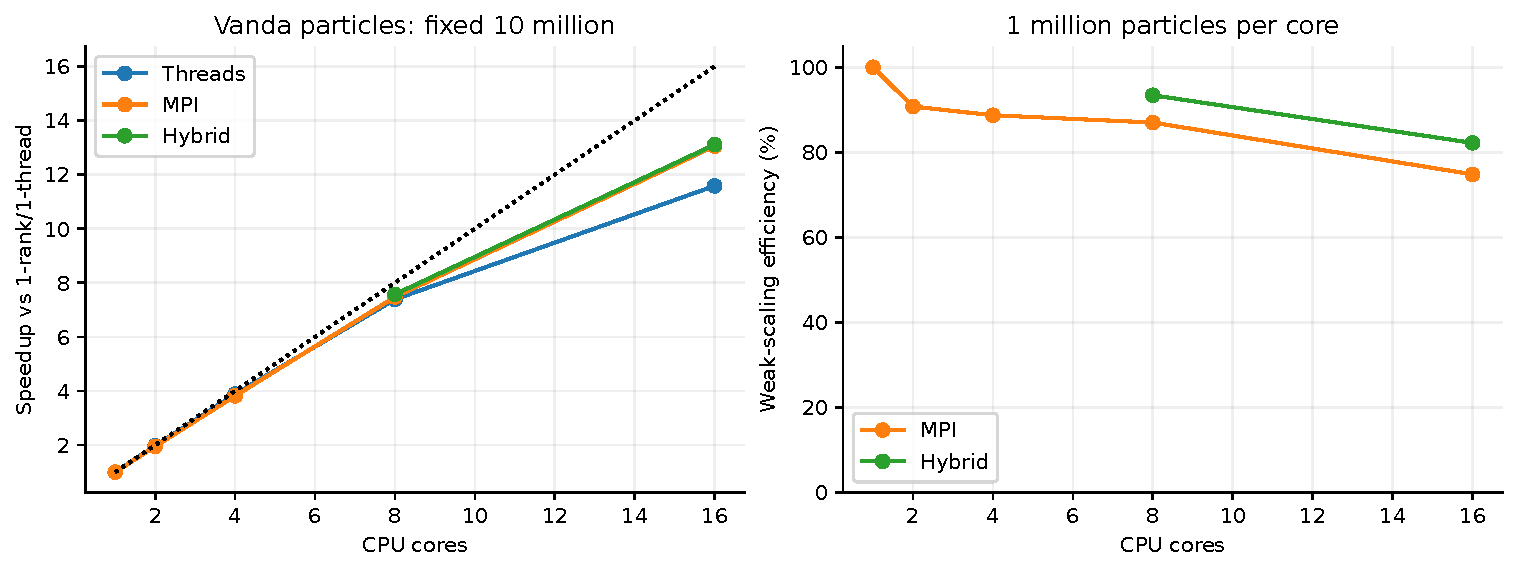
\includegraphics[width=\linewidth]{particle_scaling.pdf}
\caption{Single-node particle strong and weak scaling. Weak efficiency is $T_1(N_1)/T_p(pN_1)$. Each point comes from one run; hybrid layouts begin at eight cores.}
\label{fig:particle_scaling}
\end{figure}

The compact-plume case in Figure~\ref{fig:imbalance} uses 10 million particles, 100 steps and a release near a corner of the same $128\times128\times32$ domain. On 16 cores, $1\times16$ takes 6.38 s, $4\times4$ takes 23.07 s and $16\times1$ takes 63.40 s. The maximum-to-mean particle-count ratio reaches 13.21 with 16 ranks. Static spatial partitioning leaves many cores waiting while a few ranks own the plume.
\begin{figure}[H]\centering
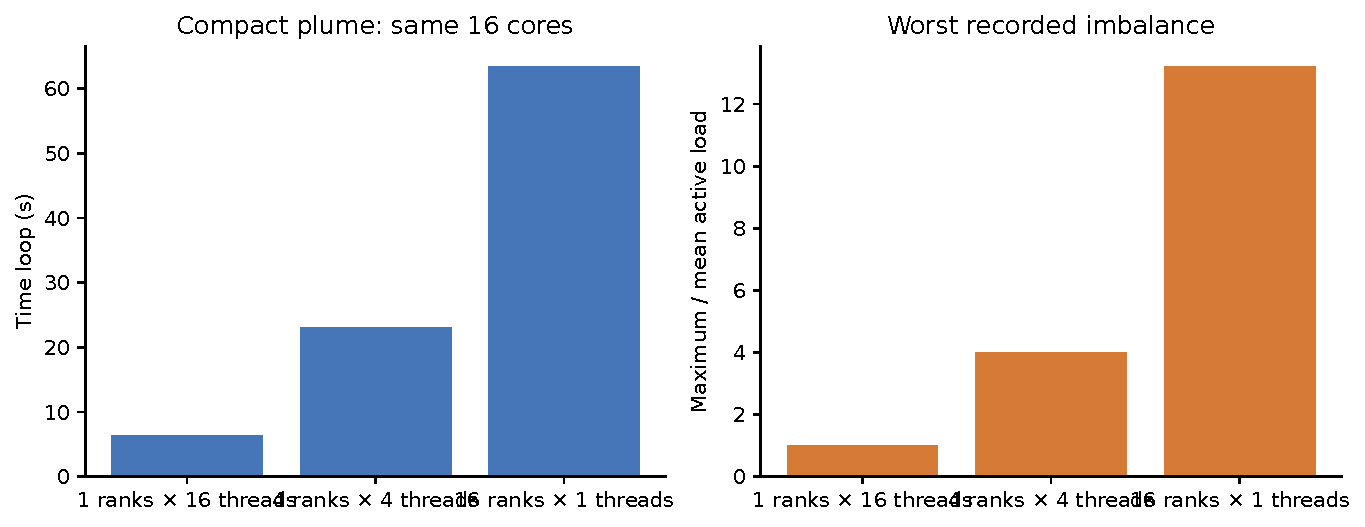
\includegraphics[width=.93\linewidth]{imbalance.pdf}
\caption{At the same total core count, a compact cloud runs faster with fewer MPI ranks and more threads per rank. These particle measurements use one node.}
\label{fig:imbalance}
\end{figure}

We interpret grid and particle timings within their own experiments because the workloads, baselines and machines differ. We also keep timer categories separate: the rank with the longest stepping time can differ from the rank with the longest wait.
\clearpage

\section{Multi-node grid scaling}
On 12 November we ran $512\times512\times64$ cells for 200 steps of $\Delta t=0.5$ s, using block decomposition, periodic boundaries and no concentration snapshots. Each node contributes 6 ranks $\times$ 2 threads. We used one warmup and three alternating-order repeats per configuration. Every layout passed serial/MPI field comparisons and disjoint two-core binding checks.

Figures~\ref{fig:multinode_vanda} and~\ref{fig:multinode_atlas} show the multi-node results. For these jobs, the allocated Atlas nodes use AMD EPYC 7R13 CPUs and the allocated Vanda nodes use Intel Xeon Platinum 8452Y CPUs. Both grid builds use GCC 13.3, Open MPI 5.0.3 and Kokkos 4.5.1. Communication uses OB1 with shared memory within nodes and TCP between nodes; Atlas explicitly selects \texttt{eth0} after an interface diagnostic. The results describe this TCP configuration. We could verify our allocated cores and bindings, but could not establish exclusive use of each whole node.
\begin{table}[H]\centering\small
\begin{tabular}{llrrrrr}\toprule
& & \multicolumn{3}{c}{Median solve time (s)} & \multicolumn{2}{c}{4 nodes}\\
Cluster & Exchange & 1 node & 2 nodes & 4 nodes & Speedup & Efficiency\\\midrule
Vanda & Blocking & 3.048 & 2.590 & 1.273 & 2.40 & 59.9\%\\
Vanda & Overlap & 4.943 & 2.679 & 1.914 & 2.58 & 64.6\%\\
Atlas & Blocking & 9.325 & 4.922 & 11.429 & 0.82 & 20.4\%\\
Atlas & Overlap & 10.302 & 5.342 & 6.992 & 1.47 & 36.8\%\\\bottomrule
\end{tabular}
\caption{Here $S_N=T_{\rm 1\ node}/T_{N\rm\ nodes}$ and $E_N=S_N/N$, separately for each cluster and exchange. Each baseline is a 12-core, one-node MPI run.}
\end{table}
\begin{figure}[H]\centering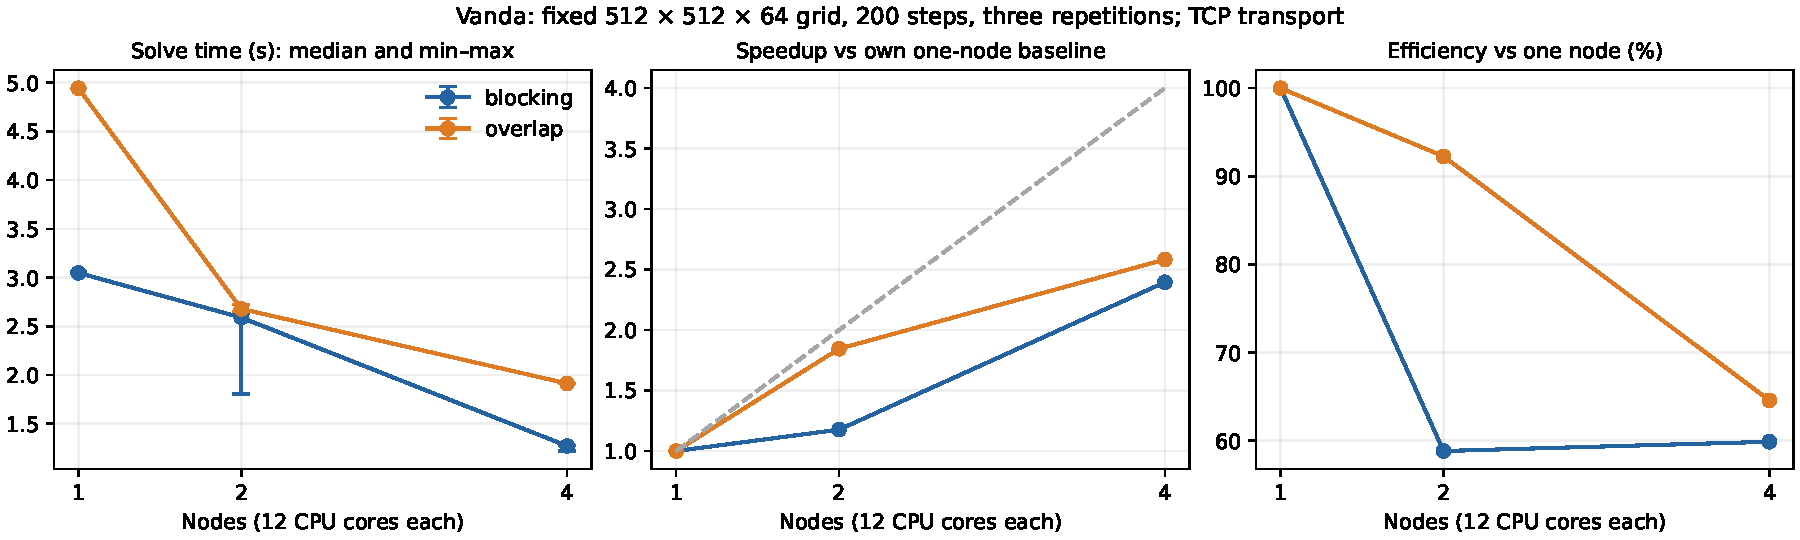
\includegraphics[width=\linewidth]{multinode_vanda.pdf}
\caption{Vanda job 1547560. Blocking finishes faster. Overlap has a larger speedup because its own one-node baseline is slower. Two-node blocking varies from 1.806 to 2.627 s; error bars retain that variation.}
\label{fig:multinode_vanda}
\end{figure}
\begin{figure}[H]\centering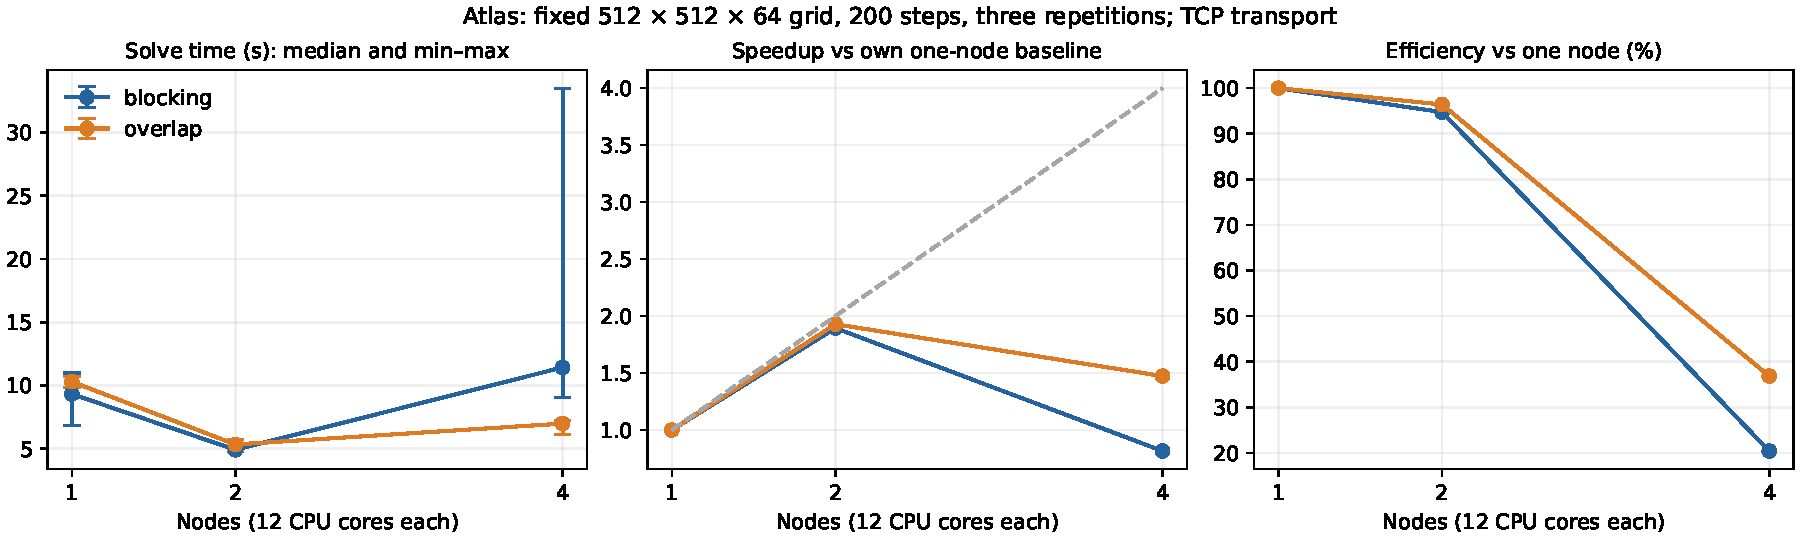
\includegraphics[width=\linewidth]{multinode_atlas.pdf}
\caption{Atlas job 1040644. Four-node blocking ranges from 9.055 to 33.497 s and its one-node baseline from 6.827 to 10.987 s. Three observations cannot identify the cause of variability.}
\label{fig:multinode_atlas}
\end{figure}
Atlas blocking update-time medians fall from 8.902 to 4.095 to 2.253 s across 1/2/4 nodes, while halo-time medians rise from 2.993 to 3.343 to 10.689 s. This points to communication and waiting as a bottleneck in the TCP run. These are separate rank maxima, so they cannot be added. Vanda scales more clearly; different hardware and allocations keep the cluster baselines separate.
\clearpage

\section{Urban inputs and experiment}
We use Zenodo record 21674773 \cite{dataset}, case \path{4_SanGeronimo_inletOutlet_vegetation_u2_alpha315}. We checked the coordinate ordering and obtained spacings $(2.3411045,2.3410716,1.9976830)$ m. We treat these samples as cell centres. The supplied mask mainly described the circular exterior, so we built a candidate building mask from horizontal STL cross-sections, checking inside/outside parity in two directions. Gaps in the STL make this mask uncertain, and the available geometry is insufficient to verify the full terrain.

The cropped domain is $641\times556\times22$ cells: 7,745,138 air and 95,574 solid cells. Its lower corner is approximately $(-699.651,-650.507,1.411)$ m. Horizontal boundaries are open; top and bottom are closed. The bottom is a simplified flat floor. Figure~\ref{fig:urban_plume_stl} places the plume within the original building geometry. Maximum absolute discrete wind divergence is $3.4865\ \mathrm{s^{-1}}$, RMS $0.02940\ \mathrm{s^{-1}}$; no divergence projection was applied. This uncertainty in the wind remains even when the pollutant mass budget closes.
\begin{table}[H]\centering\small
\begin{tabular}{ll}\toprule
Parameter & Value\\\midrule
Release centre; Gaussian width & $(150,550,12)$ m; $\sigma=3$ m\\
Initial mass; diffusivity & 1; $K=1\ \mathrm{m^2/s}$\\
Duration; saved interval & 600 s; 30 s\\
Mean horizontal wind in release core & 5.163 m/s\\
Grid execution & Atlas, 6 MPI ranks $\times$ 2 threads\\
Grid timestep & Automatic: $\Delta t\leq0.12956$ s; shortened at outputs\\
Particle ensemble & Three seeds, 100,000 particles each, $\Delta t=0.1$ s\\
Sensitivity checks & One seed at $\Delta t=0.05$ s; one at 200,000 particles\\\bottomrule
\end{tabular}
\caption{Source and diffusivity are experimental choices. The release has a clear three-sigma air core and wind directed toward the building area.}
\end{table}
\begin{figure}[H]\centering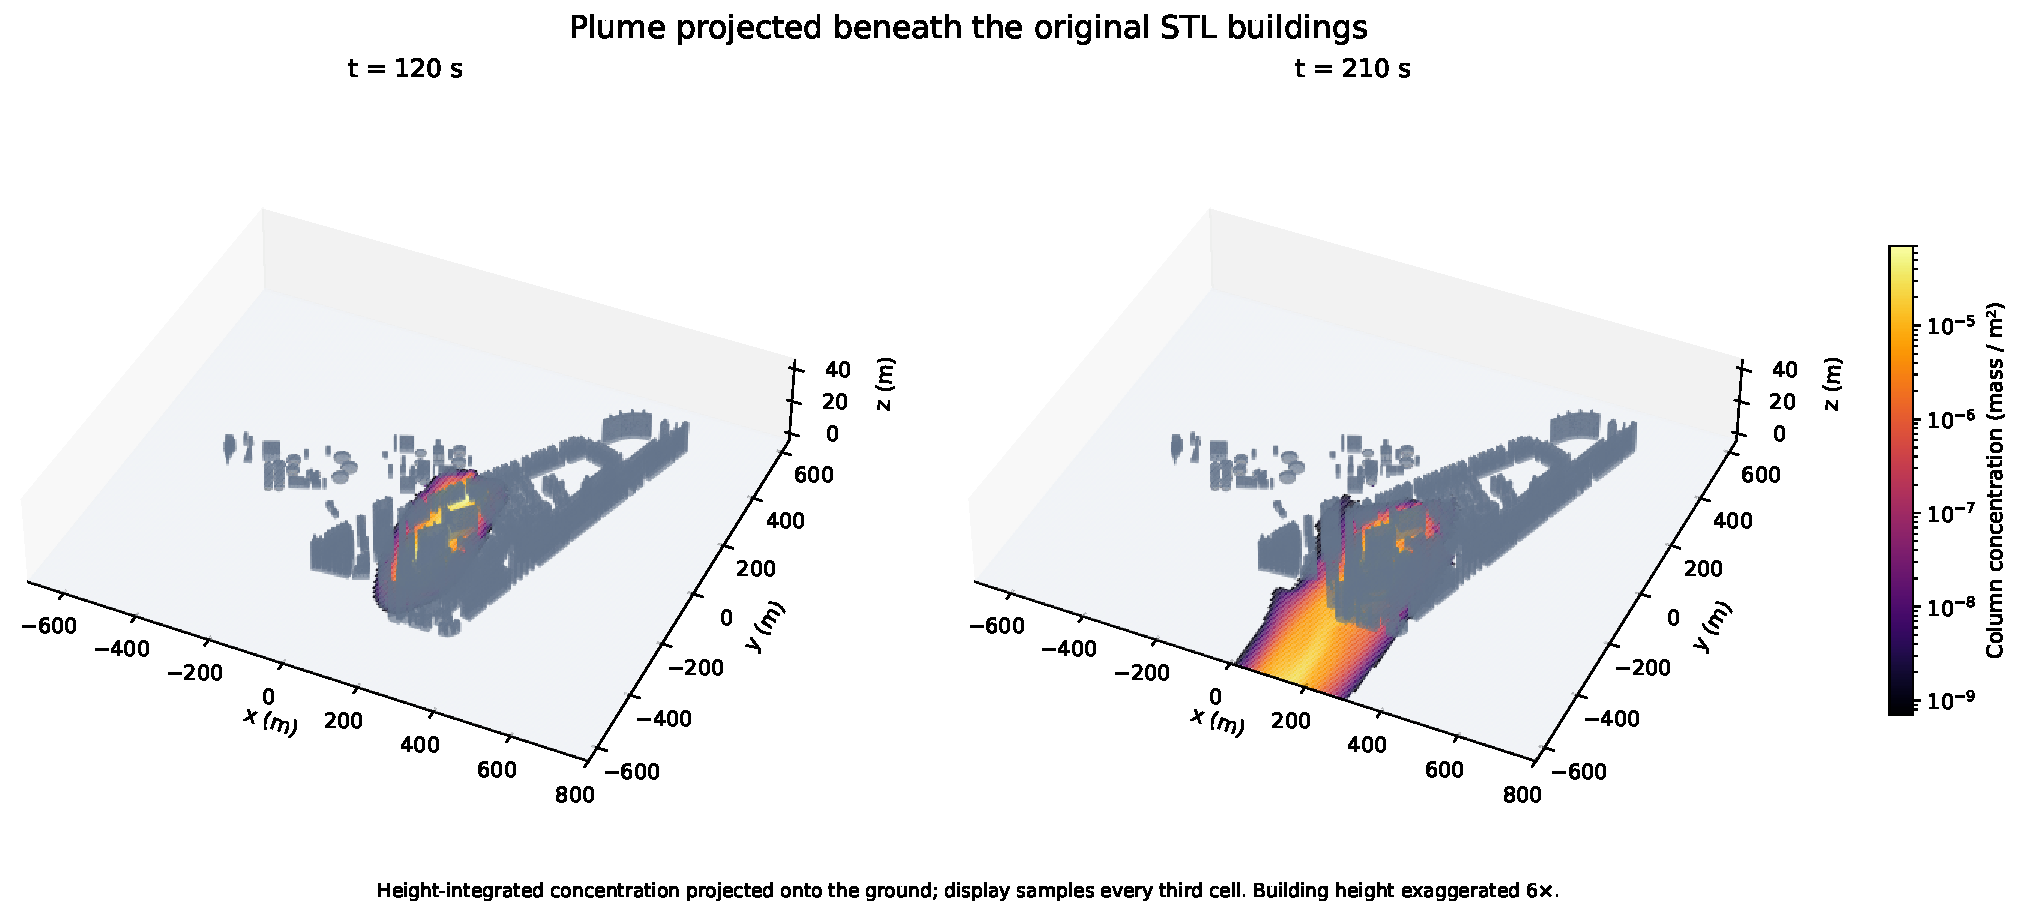
\includegraphics[width=\linewidth]{urban_plume_stl.pdf}
\caption{Original STL buildings above the actual height-integrated plume at 120 and 210 s. Height is exaggerated $6\times$; display samples every third horizontal cell. Colour shows concentration integrated over height and projected onto the ground.}
\label{fig:urban_plume_stl}
\end{figure}
\clearpage

\subsection{Three complementary urban views}
Figure~\ref{fig:urban_angle_1} shows the same 210 s field from three angles, keeping the colour scale fixed. Each view makes different parts of the building layout and plume easier to see.
\begin{figure}[H]\centering
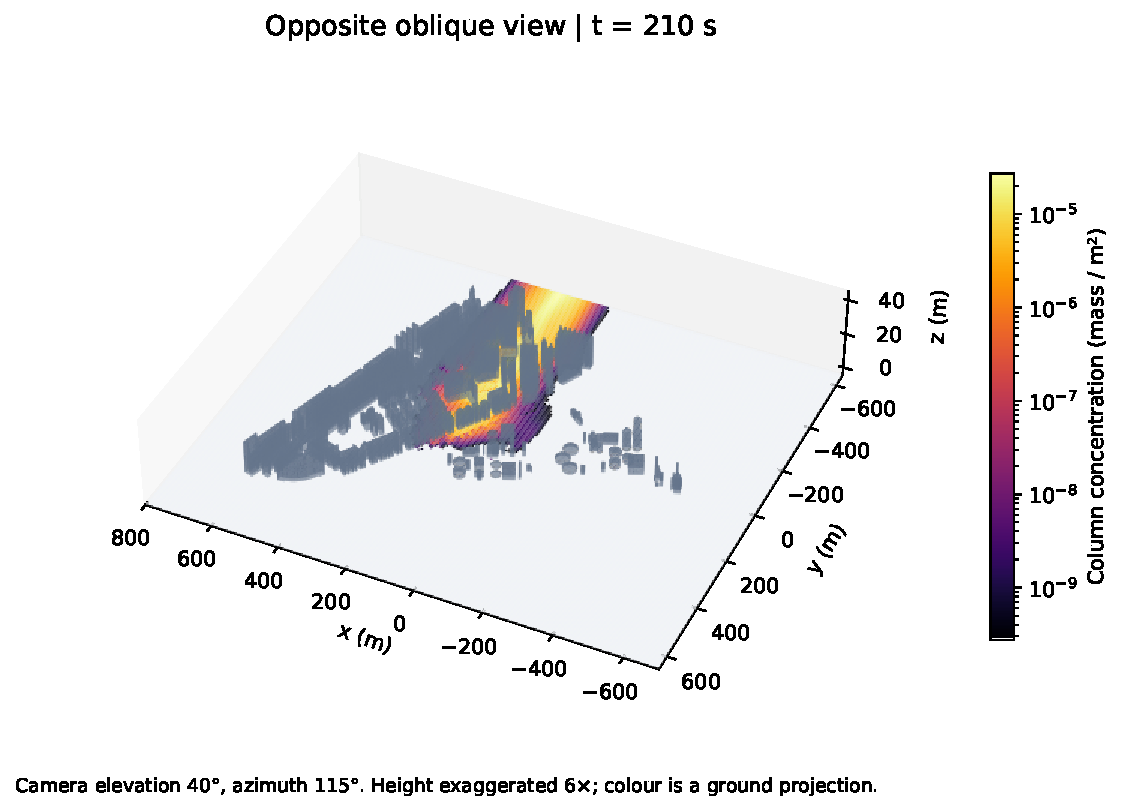
\includegraphics[width=.49\linewidth]{urban_angle_1.pdf}\hfill
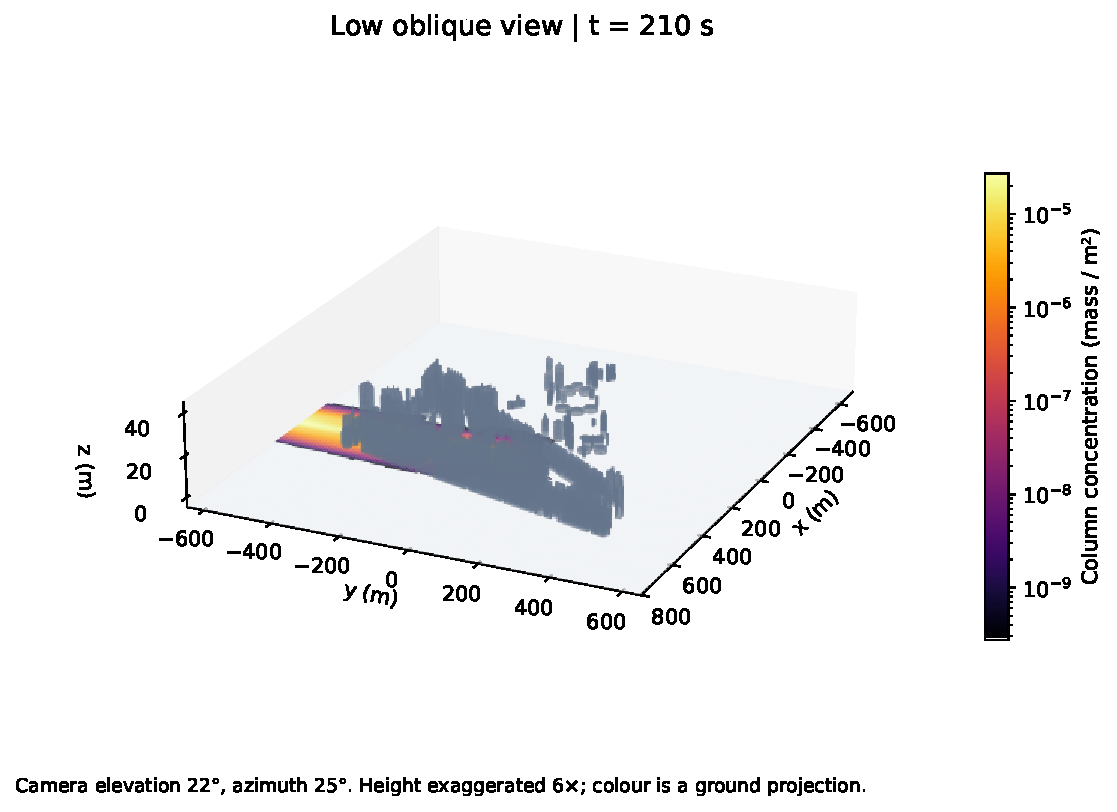
\includegraphics[width=.49\linewidth]{urban_angle_2.pdf}\\[2mm]
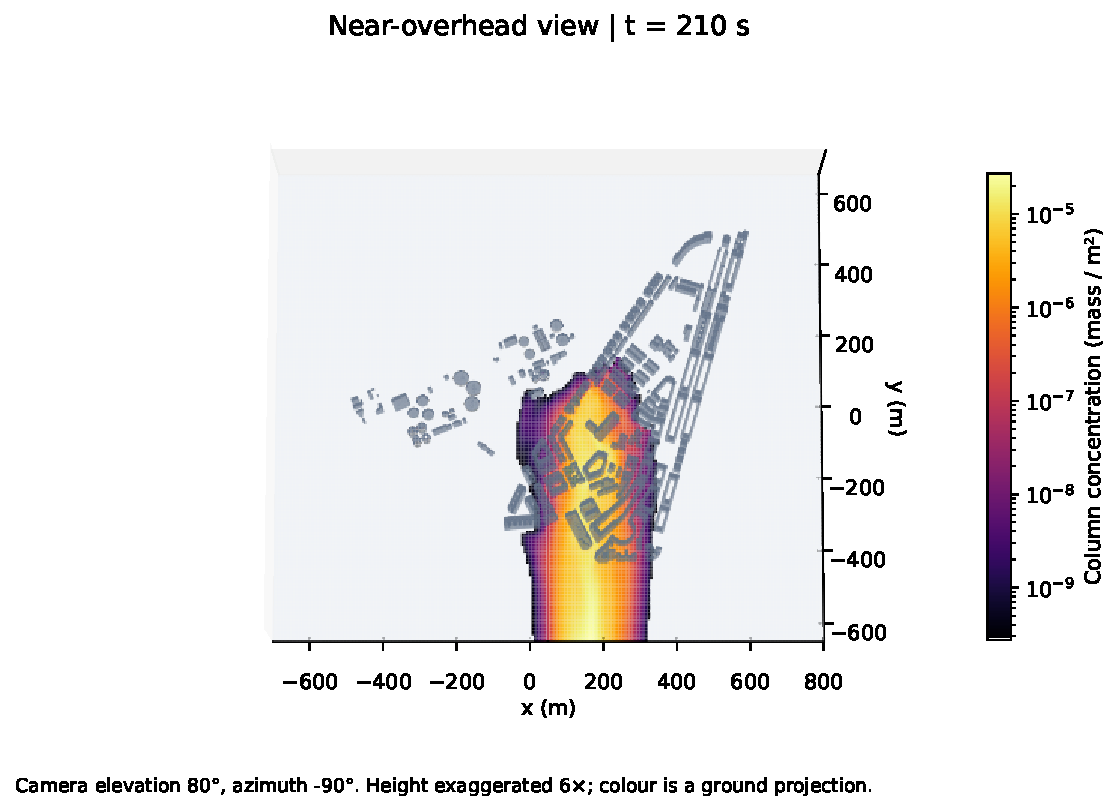
\includegraphics[width=.85\linewidth]{urban_angle_3.pdf}
\caption{Opposite oblique, low oblique and near-overhead views of the original STL and actual height-integrated concentration at 210 s. All views share one logarithmic colour scale. Height is exaggerated $6\times$ and display samples every third horizontal cell. The colours show the height-integrated plume projected onto the ground, which buildings can obscure. The overhead view makes the horizontal footprint easier to follow.}
\label{fig:urban_angle_1}
\end{figure}
\clearpage
\section{Where the plume travels}
Figures~\ref{fig:urban_plume_column} and~\ref{fig:urban_plume_xy} show column and horizontal-section output from the urban grid run. We use shared logarithmic colour scales to follow the plume over time. Pale regions are zero or below the plotting threshold; blue arrows show only the local mean release wind. Early transport follows negative $y$, then the plume spreads through the building area and leaves the domain.
\begin{figure}[H]\centering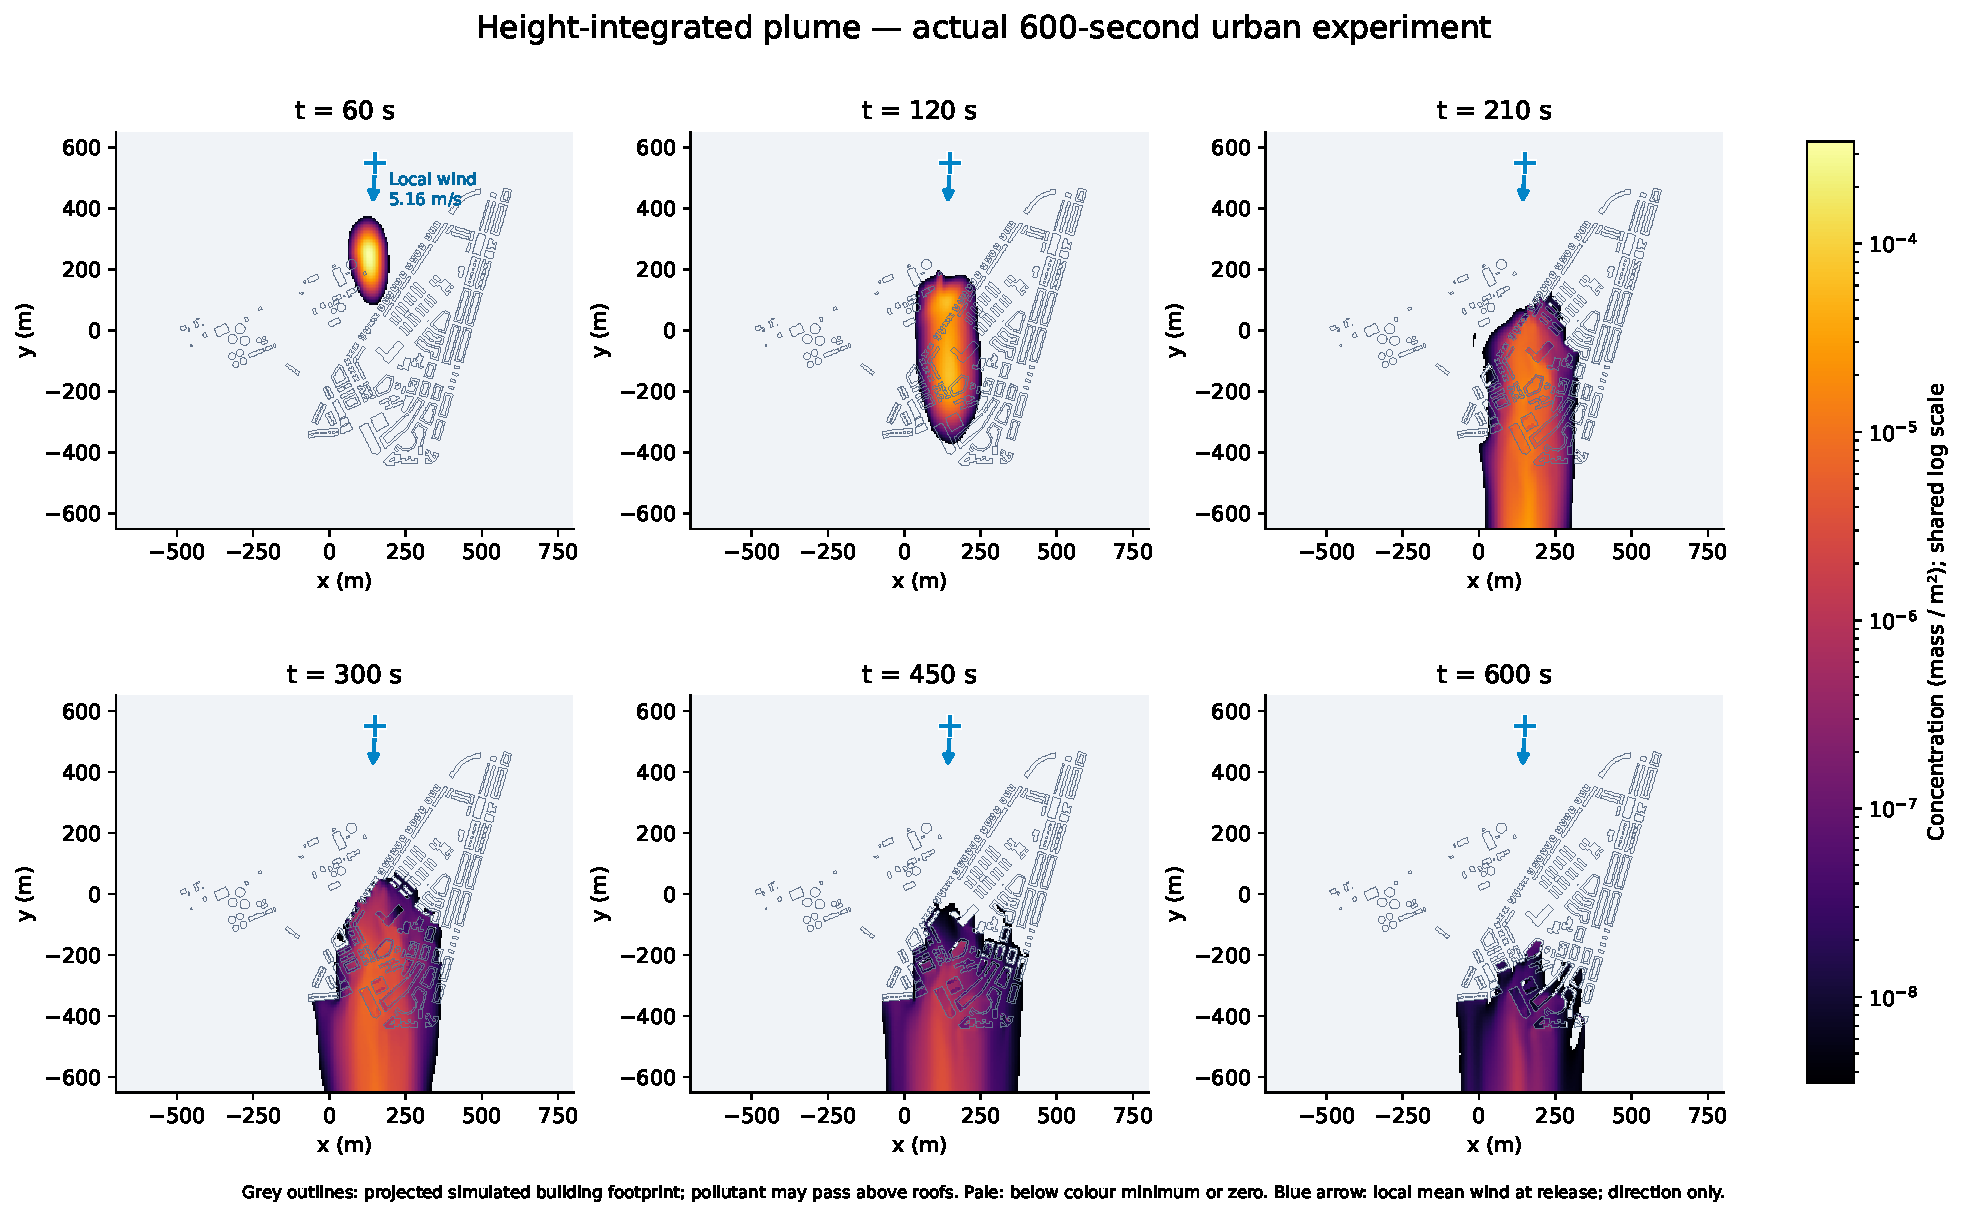
\includegraphics[width=.88\linewidth]{urban_plume_column.pdf}
\caption{Height-integrated concentration and projected solid-cell footprints. These maps show horizontal extent without selecting one height.}
\label{fig:urban_plume_column}
\end{figure}
\begin{figure}[H]\centering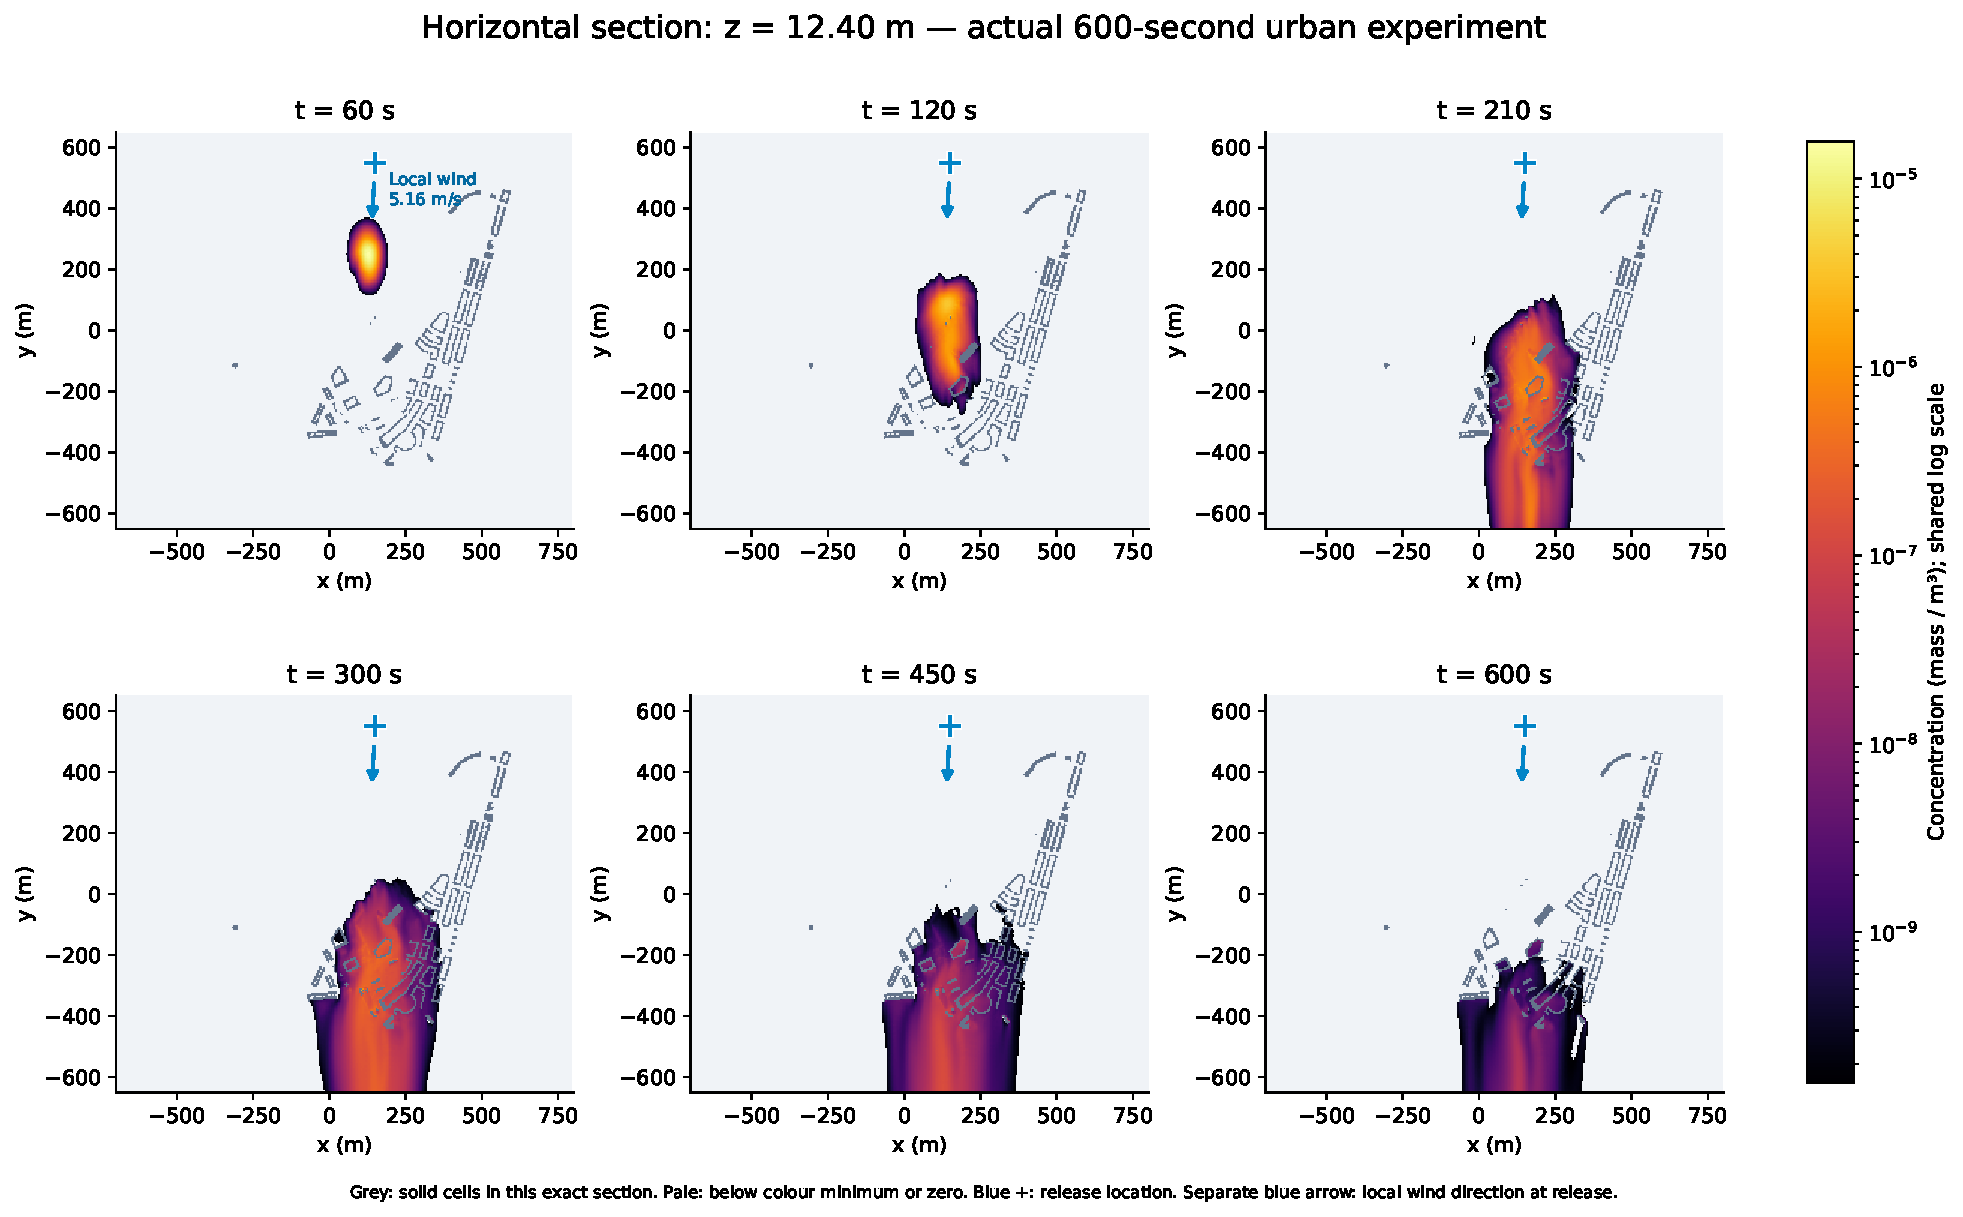
\includegraphics[width=.88\linewidth]{urban_plume_xy.pdf}
\caption{Horizontal section at $z=12.40$ m. Grey cells show solid cells at this height. The vertical coordinate follows the dataset elevation reference.}
\label{fig:urban_plume_xy}
\end{figure}
\clearpage

\section{Vertical structure and retained mass}
\begin{figure}[H]\centering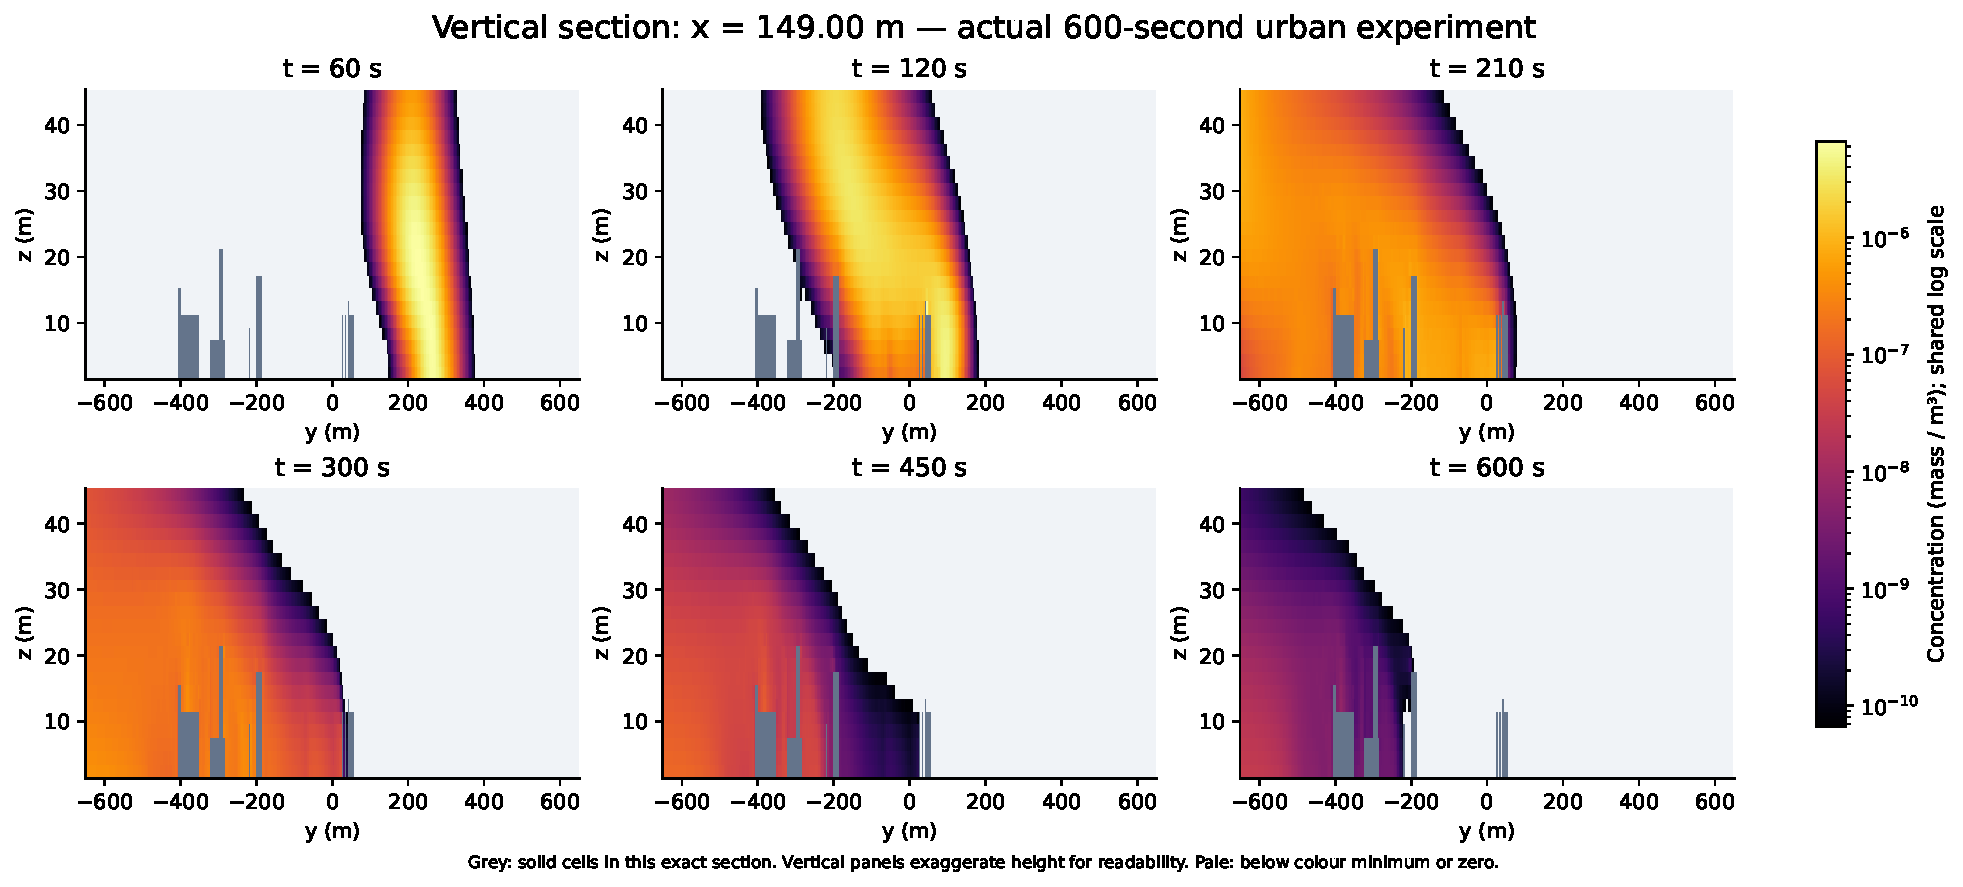
\includegraphics[width=.88\linewidth]{urban_plume_yz.pdf}
\caption{Longitudinal $y$--$z$ section at $x=149.00$ m. The plume spreads vertically while moving downstream; solids interrupt the section. Vertical scale is exaggerated.}
\label{fig:urban_plume_yz}
\end{figure}
\begin{figure}[H]\centering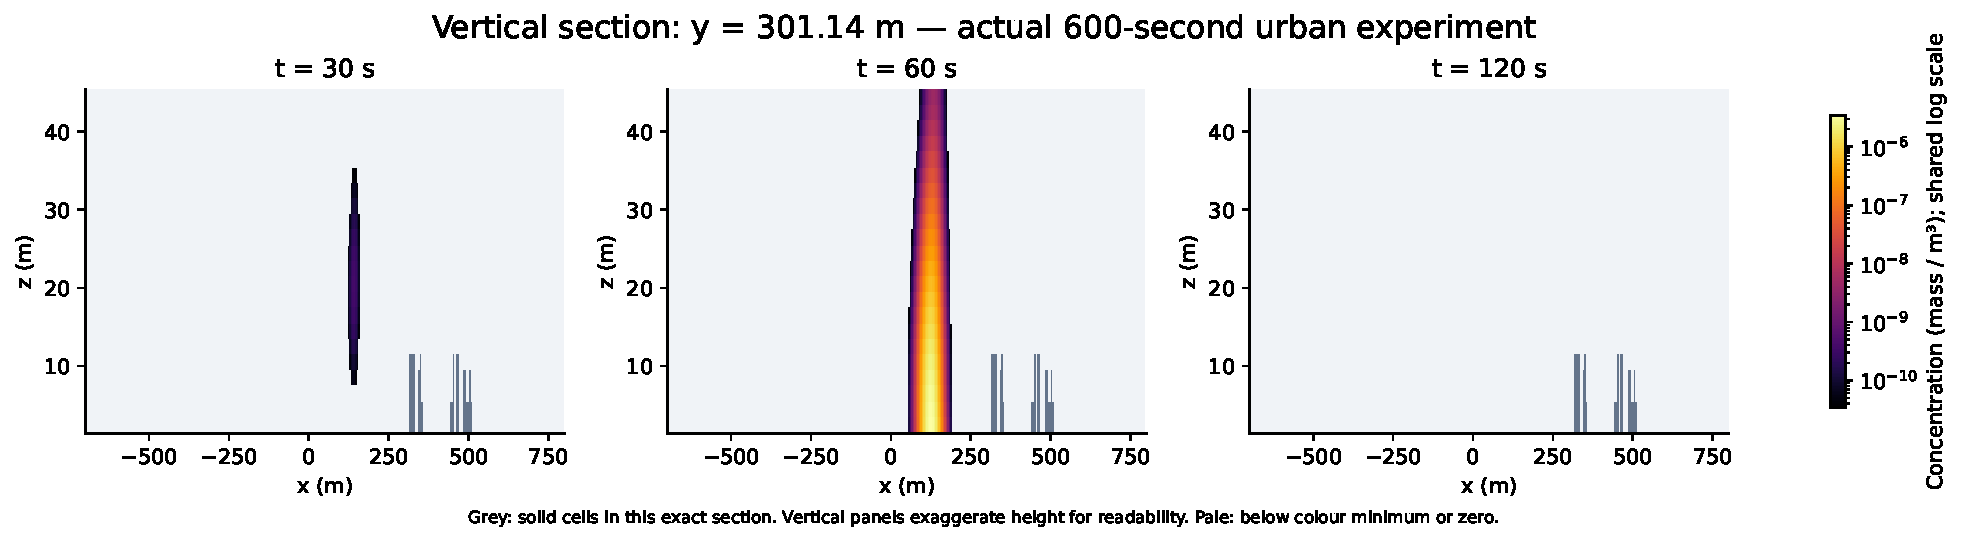
\includegraphics[width=.88\linewidth]{urban_plume_xz.pdf}
\caption{Transverse $x$--$z$ section at $y=301.14$ m. Later pale panels indicate concentrations below the colour minimum after the plume passes.}
\label{fig:urban_plume_xz}
\end{figure}
Figures~\ref{fig:urban_plume_yz}--\ref{fig:retention} show vertical structure and retention. At 600 s, grid retention is 1.39475\% of initial mass; the particle mean is 1.55433\%, with seed SD 0.06312 percentage points. Their difference is 0.1596 percentage points, or 11.4\% relative to the small grid remainder. Maximum mean-retention difference over saved times is 0.9852 percentage points at 210 s. Grid budgets close within $3.3\times10^{-13}$; particle budgets within approximately $1.1\times10^{-16}$.
\begin{figure}[H]\centering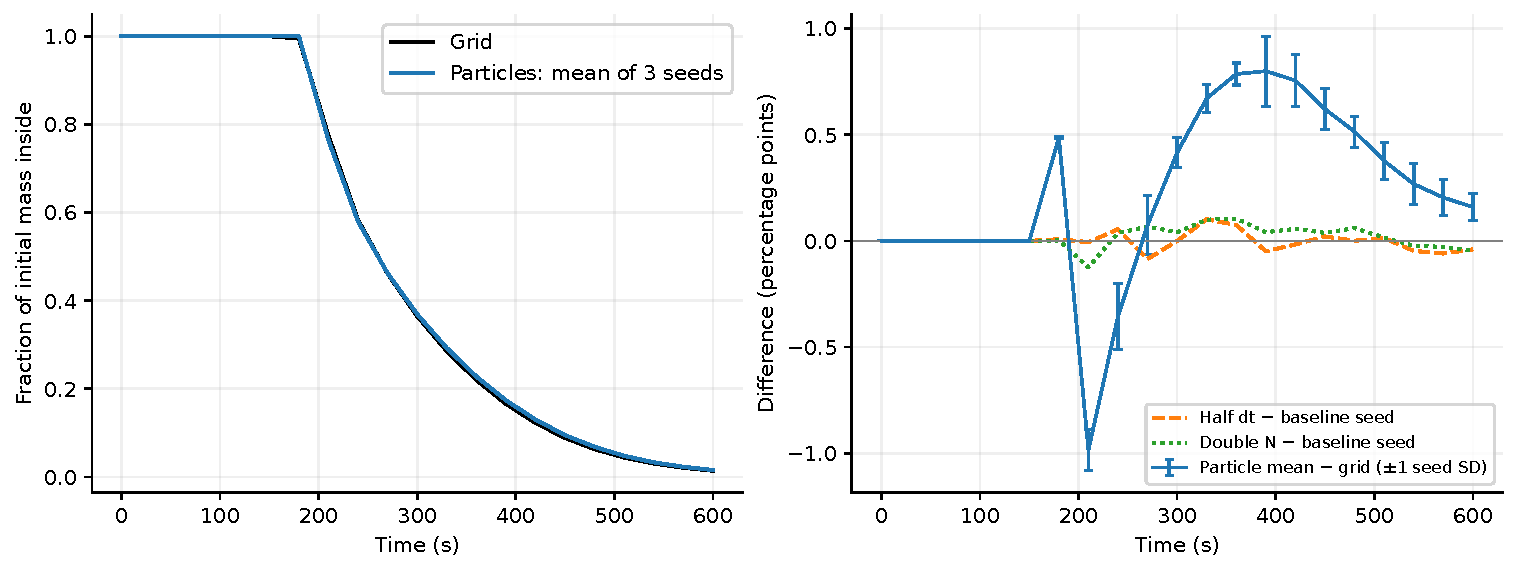
\includegraphics[width=.88\linewidth]{retention.pdf}
\caption{Retention and differences. The right-panel error bars show one sample standard deviation across the three seeds, in percentage points. Halving timestep and doubling count change retention by at most 0.102 and 0.124 percentage points in one-seed checks.}
\label{fig:retention}
\end{figure}
Interpolated grid escape reaches 50\% near 260 s and 90\% near 440 s.
\clearpage

\section{Spatial agreement depends on observation scale}
For cell or bin masses $m$, we use normalized mass discrepancy $D$ and conditional-survivor total variation $T$:
\begin{equation}
D=\frac{\sum_b|m_b^{\rm FV}-\overline m_b^{\rm P}|}{M_{\rm FV}+\overline M_{\rm P}},
\qquad T=\frac12\sum_b\left|\frac{m_b^{\rm FV}}{M_{\rm FV}}-\frac{\overline m_b^{\rm P}}{\overline M_{\rm P}}\right|.
\end{equation}
Both lie in $[0,1]$; $D$ includes mass and spatial differences, whereas $T$ compares normalized surviving shapes. We first average the three seed fields, then calculate these measures from the ensemble mean.
\begin{figure}[H]\centering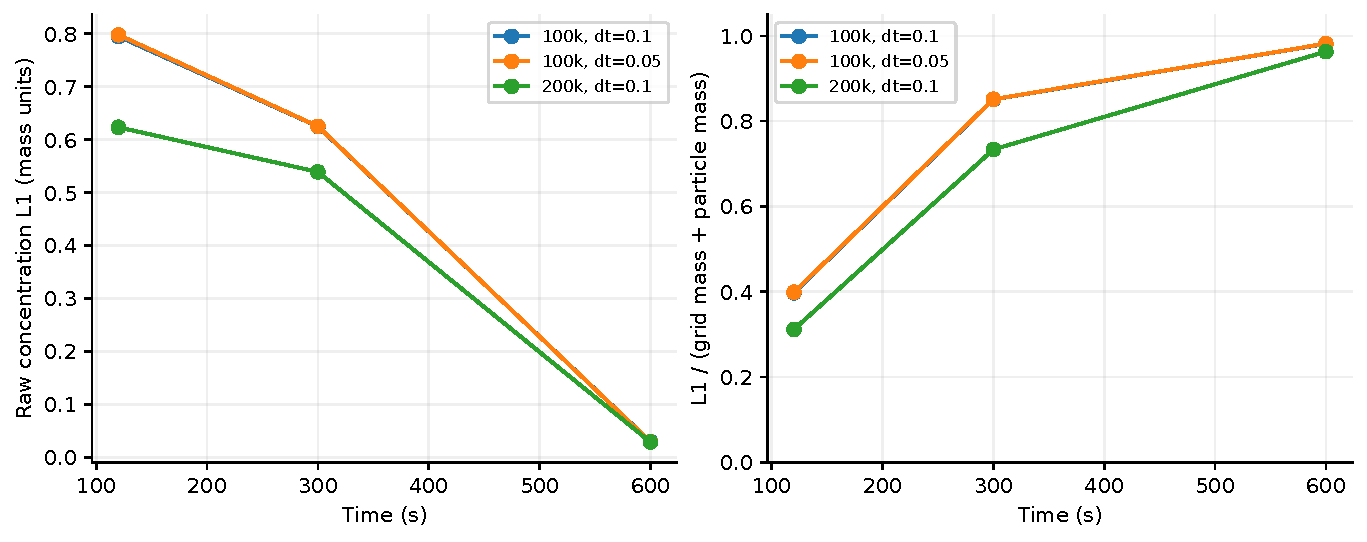
\includegraphics[width=.86\linewidth]{field_difference.pdf}
\caption{Individual-run native-cell errors. Raw L1 falls as mass escapes; normalized error remains large. The $\Delta t=0.05$ curve nearly overlaps $\Delta t=0.1$; crosses and open circles distinguish them.}
\label{fig:field_difference}
\end{figure}
Figure~\ref{fig:field_difference} shows the native-cell errors. At 600 s, about 1,500--1,630 particles per seed occupy roughly 7.8 million observation cells, leaving sparse histograms. First-order upwinding also adds numerical diffusion. For constant 1D advection, $K_{\rm num}\approx |u|h(1-C)/2$, $C=|u|\Delta t/h$ \cite{upwind}. Release-region values $|u|\approx5.16$ m/s, $h\approx2.34$ m and $\Delta t\approx0.12956$ s give $C\approx0.286$ and $K_{\rm num}\approx4.3\ \mathrm{m^2/s}$ versus $K=1$. This is consistent with the broader grid plume in Figure~\ref{fig:aggregate_maps}; Figure~\ref{fig:centroids} compares surviving-mass centres. Variable wind, walls and sampling prevent isolating each contribution.
\begin{figure}[H]\centering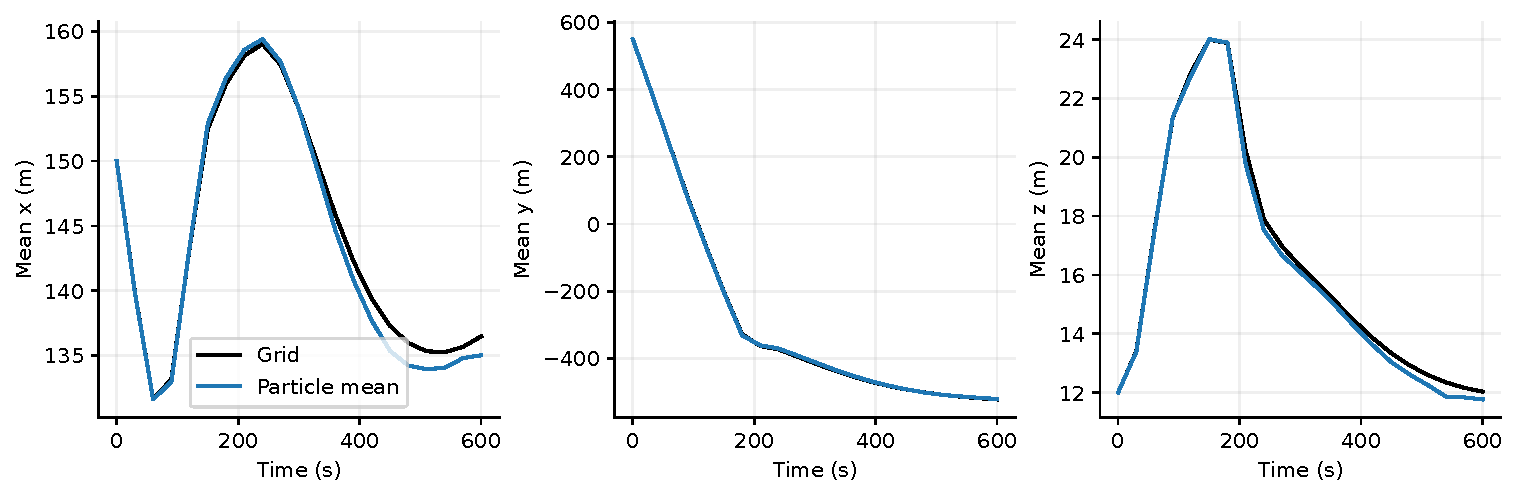
\includegraphics[width=.90\linewidth]{centroids.pdf}
\caption{Centroids of surviving mass. Each centroid uses the mass still inside the domain at that time, so the population changes as pollutant escapes.}
\label{fig:centroids}
\end{figure}
\begin{table}[H]\centering\small
\setlength{\tabcolsep}{5pt}
\begin{tabular}{rr@{\hspace{12pt}}rr@{\hspace{12pt}}rr}\toprule
& Native 3D & \multicolumn{2}{c}{\shortstack{19 m horizontal\\16 m vertical}} & \multicolumn{2}{c}{19 m columns}\\
$t$ (s) & $D$ & $D$ & $T$ & $D$ & $T$\\\midrule
120 & 0.2731 & 0.1363 & 0.1363 & 0.1115 & 0.1115\\
300 & 0.6392 & 0.0542 & 0.0525 & 0.0419 & 0.0400\\
600 & 0.9461 & 0.1555 & 0.1341 & 0.1220 & 0.0965\\\bottomrule
\end{tabular}
\caption{Grid versus the three-seed mean. Labels round 18.73 m horizontal and 15.98 m vertical widths. Column integration removes vertical differences.}
\end{table}
\clearpage

\subsection{Comparable neighbourhood-scale maps}
For Figure~\ref{fig:aggregate_maps}, postprocessing sums native-cell masses into common bins, retaining partial edge bins. The maps integrate all heights and divide by exact horizontal area. At approximately 19 m, broad plume location and extent agree more closely than native histograms suggest, although the late particle field remains patchy.
\begin{figure}[H]\centering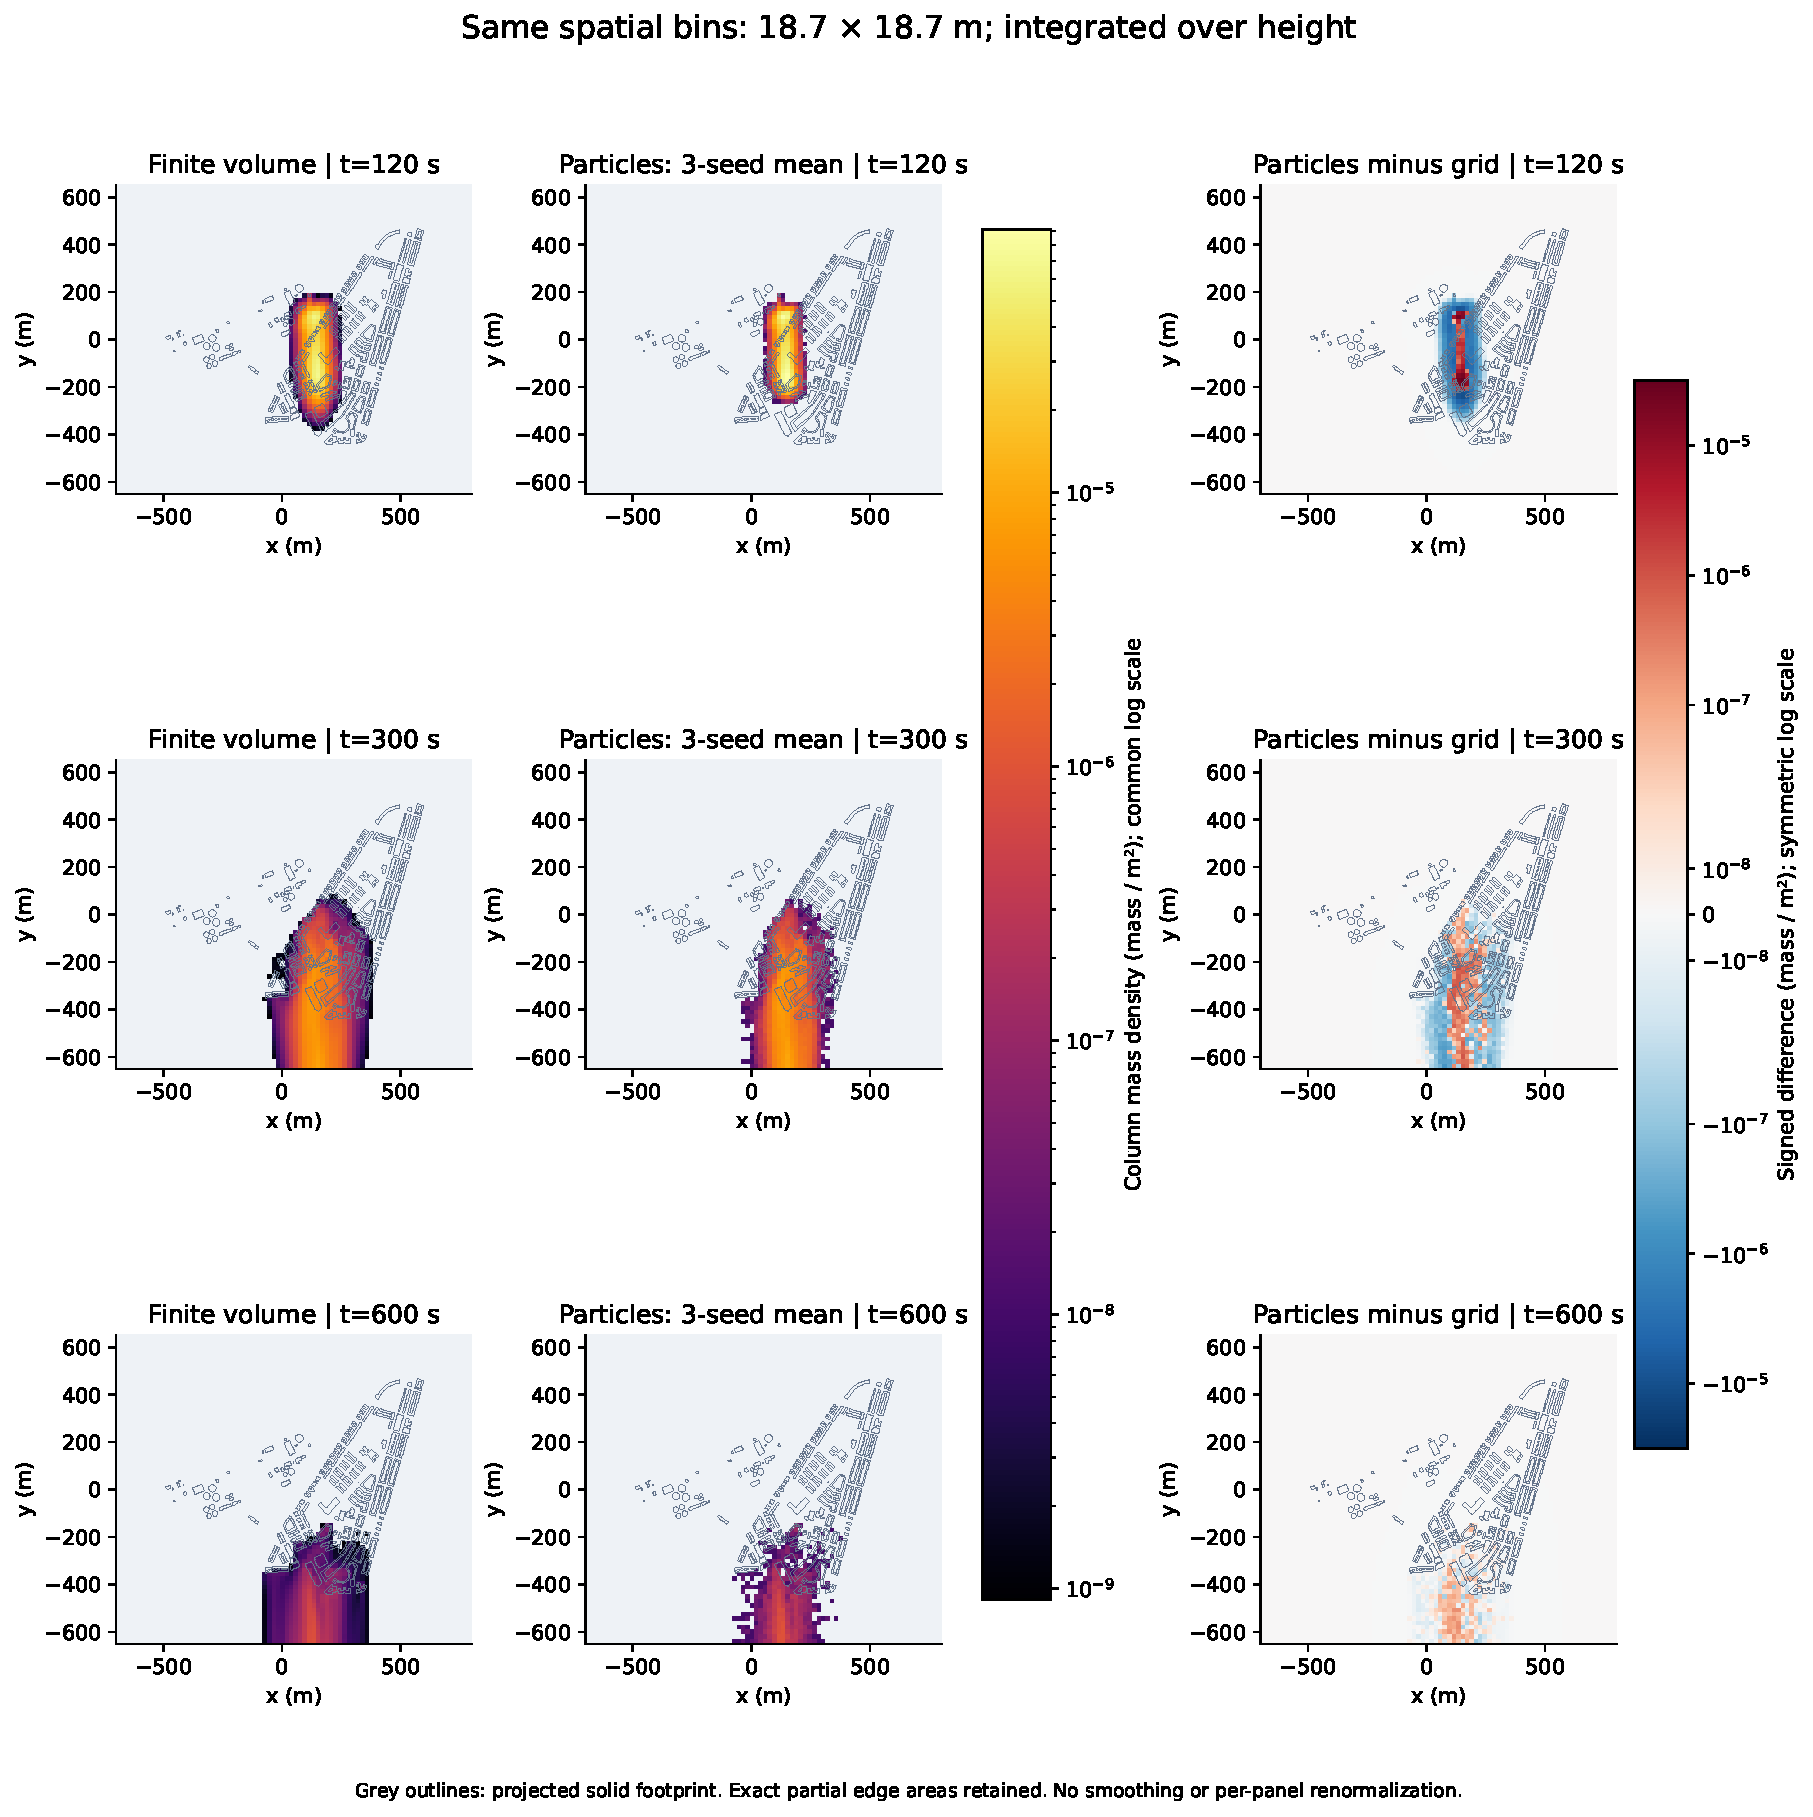
\includegraphics[width=.88\linewidth]{aggregate_maps.pdf}
\caption{At 120, 300 and 600 s: finite volume, particle ensemble mean and particles minus grid. Concentrations share one logarithmic scale; differences share one symmetric-log scale. Grey outlines show projected solids. We retain the measured mass in each panel and sum cells directly into shared bins.}
\label{fig:aggregate_maps}
\end{figure}
Figure~\ref{fig:aggregate_metrics} shows how the metrics change with bin size. Grouping neighbouring cells reduces or preserves mass L1 by construction. The coarser comparison helps us describe the broad plume location and spread. Assessing small accumulation hotspots would require more particles, grid refinement and further checks of the wind.
\clearpage

\begin{figure}[H]\centering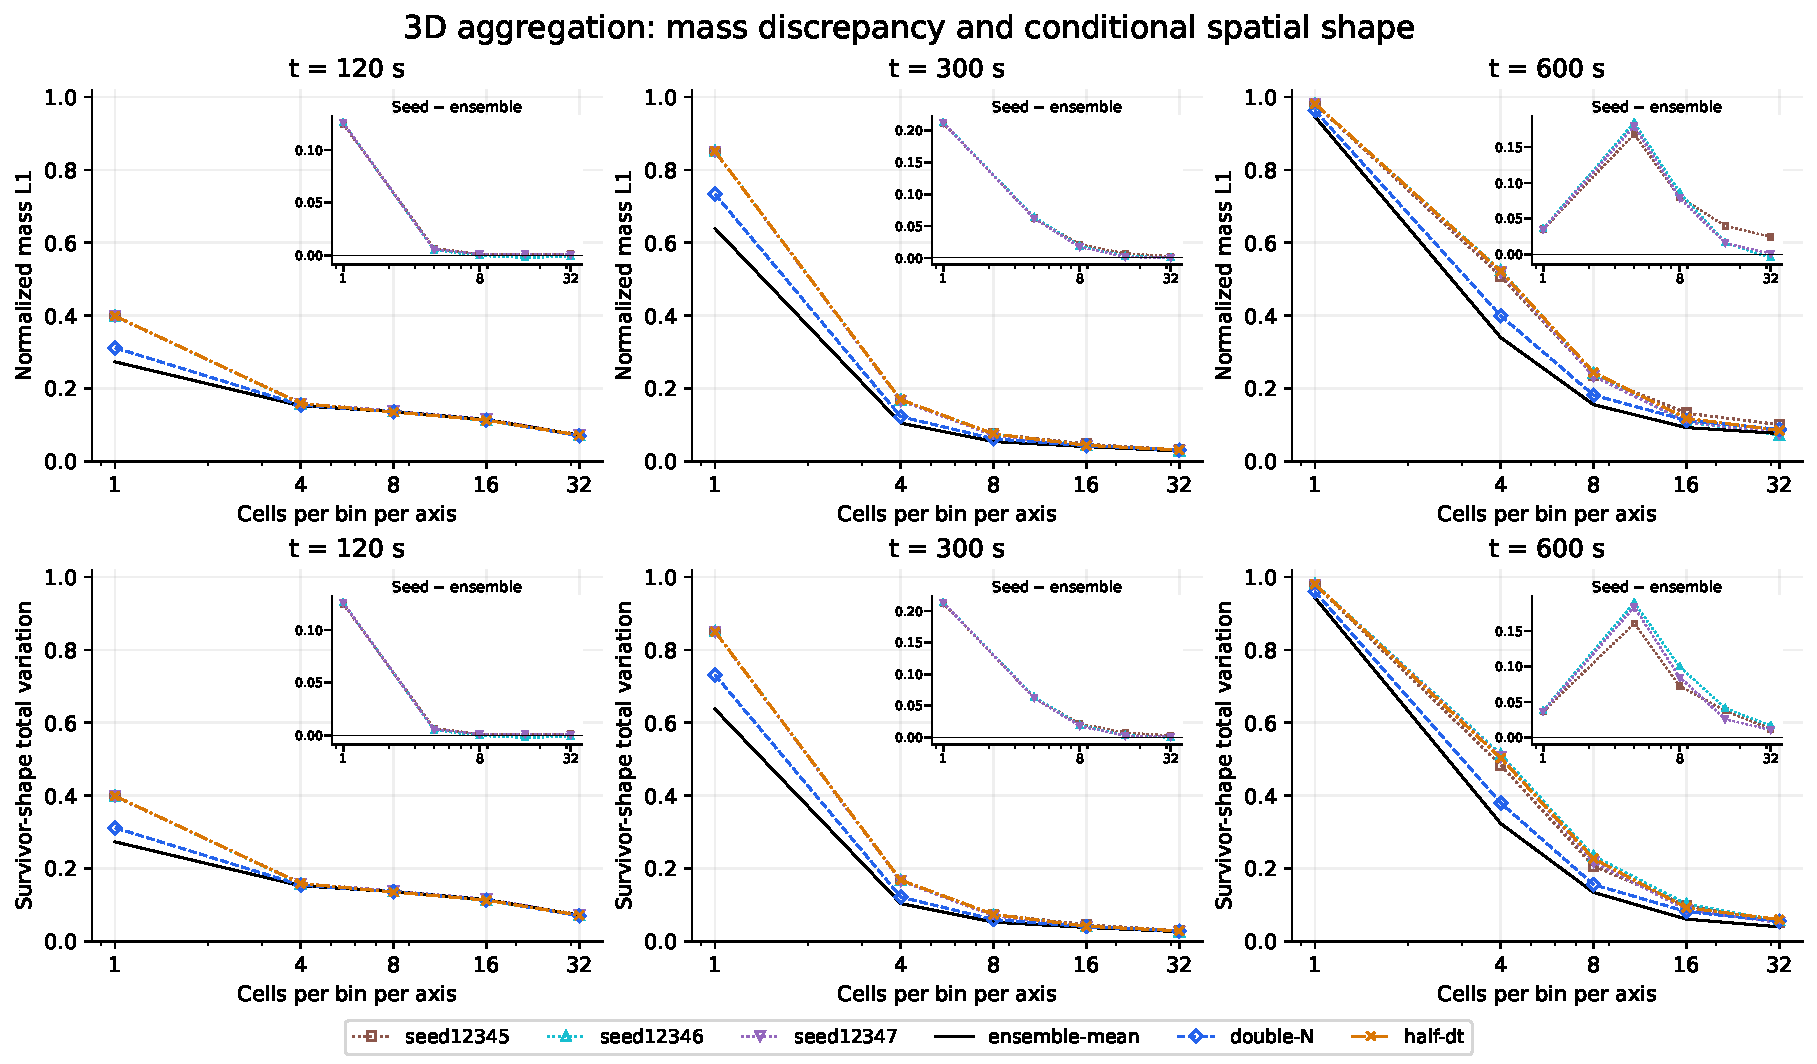
\includegraphics[width=\linewidth]{aggregate_metrics.pdf}
\caption{Three-dimensional aggregation over factors 1, 4, 8, 16 and 32. Black shows the ensemble discrepancy; coloured seed curves have an inset showing seed minus ensemble to resolve overlap. At factor 32, bins span all 22 vertical layers. Double-N uses 200,000 particles at $\Delta t=0.1$ s; half-dt uses 100,000 at $\Delta t=0.05$ s, each for seed12345. Larger bins give a coarser picture; three seeds give limited sampling information.}
\label{fig:aggregate_metrics}
\end{figure}
\clearpage
\section{Limits, lessons and reproducibility}
\textbf{Urban parallel replay.} Atlas job 1033401 used 6 MPI ranks $\times$ 2 threads and reproduced all 21 serial concentration snapshots exactly for seed 12345, with diagnostic tolerances $10^{-10}$ relative/$10^{-12}$ absolute. The 600 s run ended with 1,626 active and 98,374 escaped particles, and recorded 214,005 migrations. Maximum total time was 172.496 s; maximum output time was 103.796 s (about 60\%). Stepping time across ranks ranged from 0.0053 to 48.245 s, exposing imbalance. The corresponding serial urban run recorded 251.981 s wall time, including 157.931 s output, on a different allocation. We report these elapsed times without a controlled speedup claim. This replay checks the urban MPI implementation for this layout and seed. Measuring urban scaling would require runs at several core counts. The separate timer maxima may come from different ranks, so we report them individually.

\textbf{What we learned.} Mass budgets, analytical tests and serial/MPI comparisons check different parts of the implementation. The urban methods agreed closely on remaining mass and broad plume footprints, with larger differences at individual cells. The building mask, flat floor and divergent wind limit physical interpretation. Particle timestep changes also change the sampled random paths, so sensitivity includes both effects. Performance depended on the workload: blocking could beat overlap, and a compact particle cloud left many ranks idle. Three grid repeats and single-run particle measurements limit precise rankings. Future improvements include dynamic load balancing, shared wind storage, parallel I/O and GPU execution.

\textbf{Contributions and AI usage.} Navneet led the grid solver, urban input preparation, shared urban physics, integration and report assembly. Tridiv led the serial/parallel particle solver, particle validation and original Vanda benchmarks. AI generated and revised parts of the code, tests, scripts, figures, report text and technical reviews, and helped troubleshoot cluster runs. The authors ran cluster experiments and supplied outputs for checking; AI-assisted checks compared saved fields and timing records. We remain responsible for reviewing the work, the results and the final submission.

\textbf{Reproduction.} Public source, report and release ZIP:\par
\url{https://github.com/melarKode/dsa5208-dispersion}\par
The README covers builds, tests, examples, plots and cluster jobs. Compact evidence and the STL/mask are included; full wind/time-series and dependencies are downloaded separately. A clean M2 Pro extraction passed both CTest suites, 63 grid runs (up to 6 ranks, versus 59 Atlas runs up to 4 ranks), 72 particle MPI runs and 15 Python tests. The audit recomputes reported quantities from bundled results.
\clearpage

\section*{Evidence index}
\begin{table}[H]\centering\small
\begin{tabular}{p{.40\linewidth}p{.51\linewidth}}\toprule
Evidence & Source\\\midrule
Atlas grid validation / single-node scaling & Jobs 1031236 / 1031246; 59 validation runs / three repeats\\
Vanda particle validation and scaling & Jobs 1519104 (validation) / 1519284 (scaling)\\
Urban grid / serial particles & Atlas 1032157 / 1032182; 600 s and five particle runs\\
Urban MPI particle replay & Atlas 1033401; 21 matched fields\\
Plume views / spatial aggregation & Atlas 1033416 / 1036035; saved fields, no new simulation\\
New grid multi-node scaling & Vanda 1547560; Atlas 1040644; 1/2/4 nodes, three repeats\\
Independent local checks & Ten byte-identical refactor cases, 72 particle MPI tests, clean extraction review\\\bottomrule
\end{tabular}
\caption{The numerical evidence audit and multi-node review scripts recompute the principal reported quantities from packaged records.}
\end{table}

\begin{thebibliography}{9}
\bibitem{dataset} A. Gonz\'alez, M. I. Castillo Catal\'an, S. Chiva and S. Iserte. \emph{Distributed Training of U-Net Architecture for Data-Driven Aerodynamic Flow and Pollutant Dispersion Prediction in Urban Environments -- Dataset}. Zenodo, 2026. \url{https://doi.org/10.5281/zenodo.21674773}.
\bibitem{random123} J. K. Salmon, M. A. Moraes, R. O. Dror and D. E. Shaw. \emph{Parallel Random Numbers: As Easy as 1, 2, 3}. SC11, 2011. \url{https://www.thesalmons.org/john/random123/papers/random123sc11.pdf}.
\bibitem{upwind} R. J. LeVeque. \emph{Modified equations for the upwind method}. AMath 574 lecture 7, University of Washington, 2011. \url{https://faculty.washington.edu/rjl/classes/am574w2011/lectures/am574lecture7nup3.pdf}.
\end{thebibliography}
\end{document}
